% Version 2020-01-06
% update – 161114 by Ken Arroyo Ohori: made spacing closer to Word template throughout, put proper quotes everywhere, removed spacing that could cause labels to be wrong, added non-breaking and inter-sentence spacing where applicable, removed explicit newlines
% update – 010819 by Dennis Wittich: made spacing and font size closer to Word template, updated references and refernces style
% update – 042319 by Dennis Wittich: font size of captions set to 'small', first author names are shortened, hyphenation fixed
% update – 010620 by Dennis Wittich: Footnotes alignment set to left

\documentclass{isprs} % isprs class modified 23-04-2019 (Dennis Wittich)
\usepackage{subfigure}
\usepackage{setspace}
\usepackage{geometry} % added 27-02-2014 Markus Englich
\usepackage{epstopdf}
\usepackage{algorithm}
\usepackage{float}
\usepackage{xcolor}
\usepackage{algorithmic}
\usepackage[labelsep=period]{caption}  % added 14-04-2016 Markus Englich - Recommendation by Sebastian Brocks
\usepackage[british]{babel} 
\usepackage[hang]{footmisc}
\usepackage{indentfirst} 
\usepackage{tabularx}
\usepackage{multirow} %合并多行单元格的宏包
\usepackage{longtable} %不宽但很长的表格可以用longtable宏包来进行分页显示
\usepackage{array} %一般用于数学公式中对数组或矩阵的排版
\usepackage{makecell}% makecell命令对表格单元格中的数据进行一些变换的控制。我们可以使用 \ 命令进行换行,也可以使用p{(宽度)}选项控制列表的宽度
\usepackage{threeparttable} %制作三线表格
\usepackage{booktabs}%s三线表格中的上中下直线线型设置宏包,在这个包中水平线被教程\toprule、midrule、buttomrule。
%表头文字格式的详细设置
\renewcommand\theadset{\renewcommand\arraystretch{0.85}%
\setlength\extrarowheight{0pt}}%行距
\usepackage{graphics}%防止表格过宽
\renewcommand\theadfont{\small}%字体
\renewcommand\theadalign{rt}%行列对齐
\renewcommand\theadgape{\Gape[0.5cm][2mm]}%上下垂直距离
\newcommand{\todo}[1]{\textcolor{red}{\small\textbf{TODO: #1}}}
\setlength{\parindent}{2em}
\def\footnotemargin{1em} % added 08-01-2020 Dennis Wittich

%\usepackage[authoryear]{natbib}
%\def\bibhang{0pt}

\geometry{a4paper, top=25mm, left=20mm, right=20mm, bottom=25mm, headsep=10mm, footskip=12mm} % added 27-02-2014 Markus Englich
%\usepackage{enumitem}

%\usepackage{isprs}
%\usepackage[perpage,para,symbol*]{footmisc}

%\renewcommand*{\thefootnote}{\fnsymbol{footnote}}
\captionsetup{justification=centering,font=normal} % thanks to Niclas Borlin 05-05-2016
\captionsetup[figure]{font=small} % added 23-04-2019 Dennis Wittich
\captionsetup[table]{font=small} % added 23-04-2019 Dennis Wittich

\begin{document}

\title{Multi-Training Based Recognition of Urban Green Cover on Multi-Temporal High Resolution Remote Sensing Images}

% KAO: Remove extra spacing
\author{
 Shenghua Wan\textsuperscript{1}, Pengfeng Xiao\textsuperscript{1}\thanks{Corresponding author}, Wenye Wang\textsuperscript{1}}

% KAO: Remove extra newline
\address{
	\textsuperscript{1 }Department of Geographic Information Science, Nanjing University, Nanjing, Jiangsu 210023, China\\
}

% If the corresponding author is NOT the final author, always add a % space before the subsequent comma, i.e.
% first author name\textsuperscript{a,}\thanks{Corresponding author} , % second author name \textsuperscript{b}, etc.
% thanks to Niclas Borlin 05-05-2016


\commission{VI, }{VI} %This field is optional.
\workinggroup{VI/4} %This field is optional.
\icwg{}   %This field is optional.

% KAO: Use times symbol
\abstract{
	Urban green space plays a crucial role in the construction of ecological city and livable 
	environment. The monitoring of urban greening information is of great significance to urban 
	management. Multi-temporal high-resolution remote sensing images are important data sources 
	for urban green cover information updating, while effectively identifying vegetation 
	information from these images is one of the key part which often faces many challenges. 
	Firstly, to achieve good results by supervised learning, large scale training samples are 
	usually needed. However, the labeling of training samples on remote sensing images is 
	time-consuming and laborious. Secondly, because of the data distribution shifting from 
	time to time, the training samples under a single time-phase can not be directly applied 
	to other phases, which results in a great waste of labeled samples. It is necessary to 
	construct the framework of information extraction of vegetation and other kinds of ground 
	objects in multi-temporal images in order to deal with such problems. Based on 
	semi-supervised learning and high resolution remote sensing images under multiple time 
	phases, an algorithm for ground object classification is proposed. This method 
	simultaneously solve the dataset shift and ill-posed problem of multi-temporal remote 
	sensing image classification, and effectively improves the accuracy of small sample 
	training on each image while ensuring the consistency of classification results. It brings 
	a new mode to the information extraction of multi-temporal remote sensing images.
}

\keywords{Multi-training, Multi-temporal, vegetation recognition, High spatial resolution image}

\maketitle

%\saythanks % added 28-02-2014 Markus Englich

\section{Introduction}\label{Introduction}

% KAO: Sloppy spacing ensures non-overfull lines. Can be removed if this is not an issue.
\sloppy

Vegetation, as an important part of urban ecological landscape, plays a key role in air filtration, microclimate regulation, noise reduction, and water quality amelioration (P. Bolund and S. Hunhammar, 1999). Therefore, inventorying the spatial distribution and detailed information (e.g., species and habitat types) of urban green cover is imperative in decision-making about natural landscape management and planning( D. Wen, 2017). 
Remote sensing image is an important resource to extract urban vegetation cover information. The commonly used data sources are Landsat, MODIS, and now very high-resolution remote sensing images bring new impetus to the monitoring of urban vegetation. VHR remote sensing data have shown great potential in detailed urban classification (X. Huang and L. Zhang, 2013), and can be utilized to extract both the locations and the corresponding attributes of green cover( D. Wen, 2017).

The property of high spatial resolution provides more accurate vegetation extraction results and sufficient data in time phase. The abundant data of multi-temporal remote sensing images provide strong support for the classification of land cover, which can distinguish land cover objects more effectively than the single-phase classification. However, the classification of remote sensing images under multi-temporal conditions is mainly faced with these problems: (1) Using supervised learning method to extract vegetation information can obtain better results, while it also needs a large number of labeled samples .(2) Because the spectral information of vegetation are influenced by seasonal change, the labeled samples in one phase can not be directly applied in another phase. Therefore, multi-temporal remote sensing images bring more opportunities and challenges to urban vegetation extraction.
To solve the problem of land cover classification based on multi-temporal remote sensing images, some researchers apply machine learning methods to stacked multi-temporal data which classify land cover objects on single time phase in isolation and do not consider the correlation between different time phases.
With the development of deep learning techniques, some research combined with recurrent neural network (RNN) in deep learning to mine remote sensing image information on time series for the reason that RNN has the advantage to process time series data, but at meantime it brings huge time cost and needs the great number of labeled samples.

Domain adaptation is a representative method of transfer learning whose data contains source domain and target domain. The purpose of this method is to apply the classifier trained in source domain to target domain and make full use of the knowledge learned in source domain. This kind of method is usually based on sample migration, feature-based migration or model-based migration. This method has been widely used in remote sensing field such as remote sensing image classification, land use/land cover classification result map updating. It takes advantage of the feature that the object on similar temporal will not change significantly. But the direct problem is that to be learned well enough, a large number of source domain labeled samples are also needed to train classifiers.
Semi-supervised learning is another kind of promising approach. In most time, the number of unlabeled samples is sufficient which will implement data information and semi-supervised learning is proposed to solve how to utilize the unlabeled data. The main idea is to train an initial classifier by using labeled training samples, and then add new training samples into the training set according to certain rules in the training process, and iteratively make the classifier update. A semi-supervised learning field can be divided into four methods, generative methods (Shahashahani and Landgrebe, 1994), low-density separation algorithms, such as TSVM (Joachims, 1999; Vapnik, 1998), graph-based methods (Jordan, 1998), divergence-based methods, such as cooperative training (Blum and Mitchell, 1998). These semi-supervised learning methods have achieved remarkable results in machine learning related tasks, and many scholars use these methods to classify remote sensing images between phases. A modified TSVM classifier is designed for addressing ill-posed remote-sensing problems(Chi, 2005). Some used Tri-Training method to execute LULC classification(Zhou and Li, 2005). Some have used semi-supervised fuzzy C means clustering method to dynamically extract vegetation information in time series remote sensing images. But due to the complexity of the remote sensing image data’s distribution, such as homomorphism, and the migration of data distribution, these methods can not achieve ideal results directly. Hence, several of researchers have proposed some strategies to extend co-training algorithms from single image classification to multi-temporal ones so that the problem of migration of data distribution can be solved. Cooperative training method is applied to identify and extract snow cover in temporal remote sensing images(Zhu and Xiao, 2016).

This work proposes a method for land use types classification based on a small number of samples on multi-temporal remote sensing images. Based on the idea of semi-supervised learning, the remote sensing image data of multiple phases in the same year is selected. After pre-processing correction and registration, the corresponding four classifiers are used. Under the training condition of a very small number of samples, the prediction probability map of each time is generated iteratively, and the invariant value of the same sample is calculated by combining the probability output value of the four classifiers. Note that this value can essentially refer to the change of a single pixel, and point out the category of the pixel at meantime. According to the setting threshold, we randomly select a certain number of samples from each class added to the training set, and the classifiers train repeatedly until the iteration was completed.
There are three main contributions in our paper. Firstly, the proposed method can utilize information from multi-temporal remote sensing images and classify the land use types well especially the vegetation. Then, this method solved the problem that different phase’s data distribution shifts greatly and we convert it to the power of model’s classification. Finally, this method can view different phase’s data globally, and make progress both on the accuracy and consistency compared with previous related approaches.
The rest of this article will be organized in six sections: the section 2 is the introduction of methods, the study area and data are introduced in section 3, the experiments are represented in section 4, the presentation and comparative analysis of the results are in section 5, and the discussion and summary are described in section 6, 7.


\section{Methodology}\label{sec:Methodology}

\subsection{Base classifier}\label{Base classifier}

Random forest is a widely used method in machine learning which can be regard as ensemble of 
decision tree classifier. It adopts random selection on data and features, constructs many 
independent decision trees, and combines the results of all decision trees. Random forest can 
improve the prediction accuracy without significant increase in computation. The following is 
the process of random forest :(1) Assuming that there are N samples, N samples are randomly 
selected to train a decision tree as a sample at the node of the decision tree root. (2) When 
each sample has M attributes, the nodes of the decision tree are divided when cracking, m 
attributes are randomly selected from the M (m is much less than M), and then an optimal 
attribute is selected by the method of decision tree selection. (3) The decision tree formation 
process splits repeatedly according to (2) until it can not. (4) Build a large number of 
decision trees according to (1) (2) (3) to form random forests. Following the above procedure, 
a random forest model with excellent performance can be trained.

In our algorithm design, random forest classifier is not the only feasible base classifier. 
In fact, in our algorithm, the base classifier needs to satisfy that can give the probability 
of which category each sample belongs to. It is convenient for the following step to select 
samples with certain probability. So the key feature of the base classifier is that it can 
predict the probability distribution of the sample set, and our method can be extended by 
using different base learners without too many constraints.



\subsection{Multi-Temporal extensions of base classifier}\label{sec:Multi-Temporal extensions of base classifier}

\begin{figure}[ht!]
	\begin{center}
			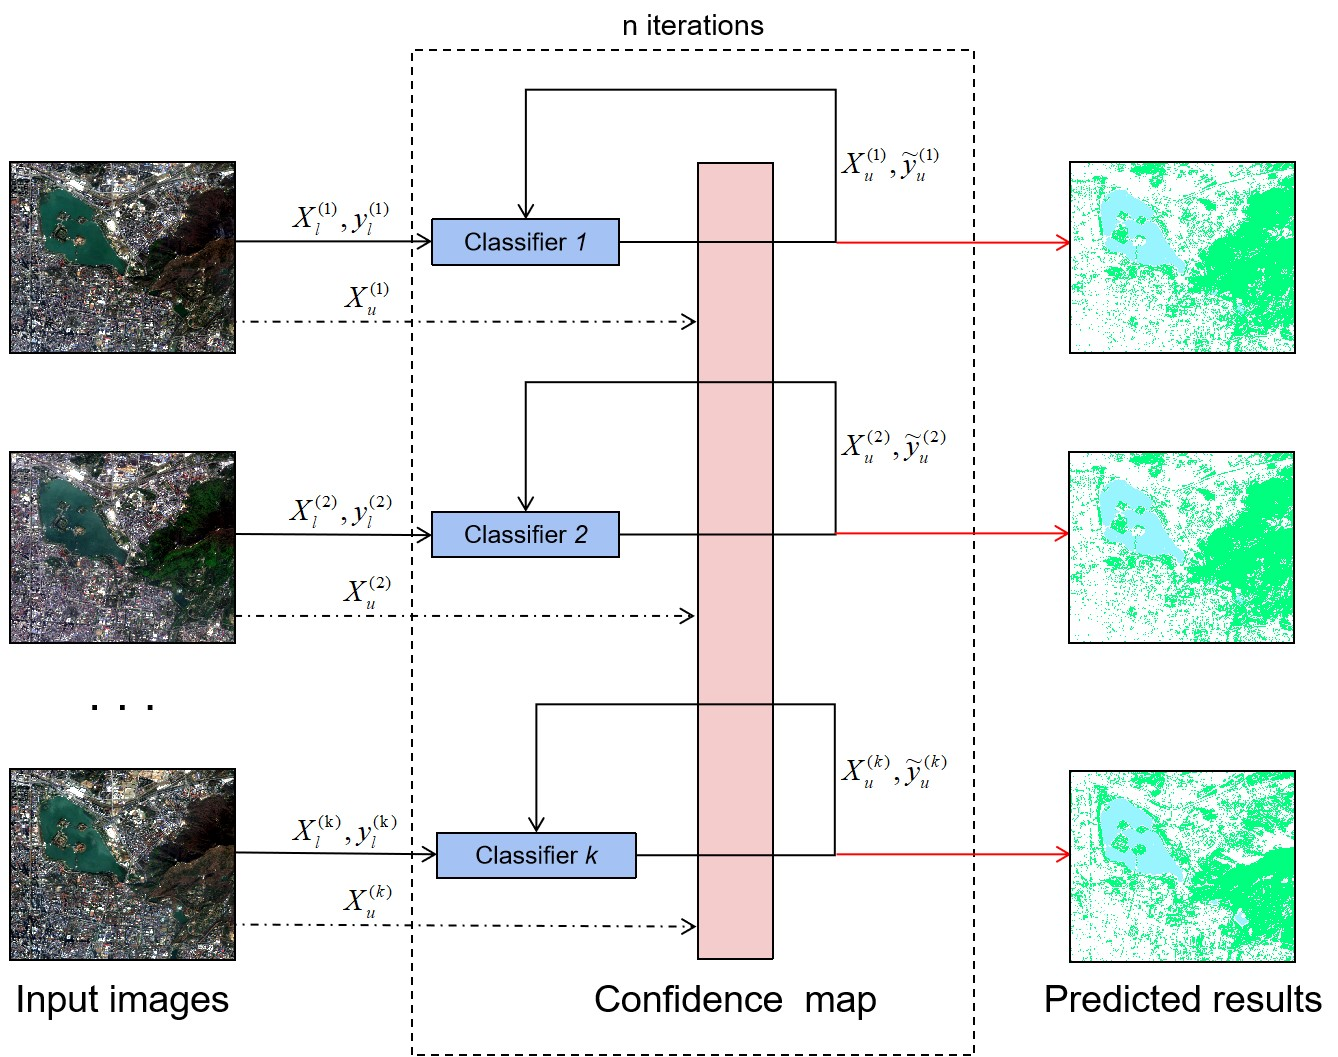
\includegraphics[width=1.0\columnwidth]{figures/images/trainClassifiers1.jpg}
		\caption{Figure placement and numbering}
	\label{fig:figure_placement}
	\end{center}
\end{figure}

Under the setting of multi-temporal, a cascade mechanism is needed to make effective use of the time-phase related information, so that the classifiers under each time phase can communicate with each other during training and share the information obtained in each own domain. The assumption of the whole problem is that most of the samples’ category have not changed during short time. Based on this premise, our algorithm allows the classifier to learn the data distribution under their respective time phases. Then after each round of learning, the communication of information is carried out which is divided into two stages, evaluation and update. The purpose of the evaluation is to fuse all the classifiers’ prediction and compute the confidence of the prediction categories of samples at the same position under multiple phases. The update stage is to put the samples with high confidence into the training set of each classifier. Each classifier will learn from each other in a round of communication, increasing the robustness and consistency of multiple classifiers. After finite iterations, the classification results of multiple classifiers are more consistent, while the natural difference of raw data guarantees the difference of their classifiers.


\subsection{Selection of unlabeled sample for training}\label{sec:Selection of unlabeled sample for training}

When processing multi-temporal remote sensing image data, it is inevitable to encounter data offset problem. The reasons for the inconsistent distribution of data come from various sources: (1) due to the influence of atmospheric radiation at different times, the change of position and height angle of the satellite and the imaging conditions of the satellite are quite different, which leads to the difference of remote sensing images even in the same region; (2) the influence of seasonal variation is not considered at the single phase, the objects in the images will also change in the spectral spectrum under multiple phases; and (3) for the reason of the changes of the objects themselves, the data distribution in the feature space in same area may be seriously shift, even the land cover type will change. Because of the problem of data distribution offset, if the samples in one image be applied directly in other phases, it will often lead to the problem of low classification accuracy and inconsistent classification results.

\begin{figure}[ht!]
	\begin{center}
			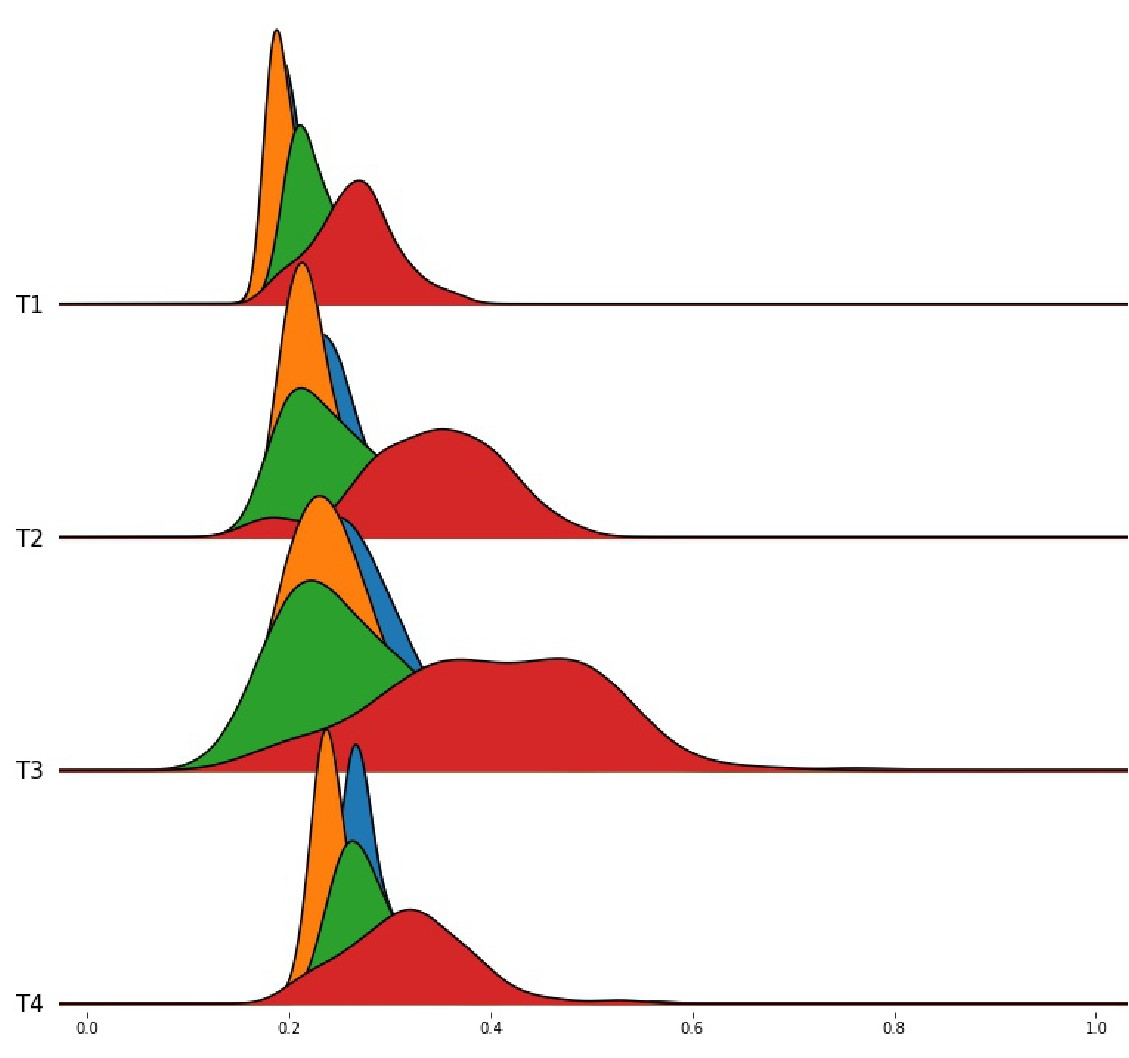
\includegraphics[width=1.0\columnwidth]{figures/images/temporal_difference1.jpg}
		\caption{Figure placement and numbering}
	\label{fig:figure_placement}
	\end{center}
\end{figure}
In order to make full use of the time-phase data information, the most important step is to determine the unchanged region and the changed region of the ground object, so that the information redundancy on the multi-temporal area can be utilized for multi-temporal training to improve classification accuracy. Most of the algorithms of multi-temporal cooperative training need to set the measurement criteria before training, divide the changed area and the unchanged area, and then train on the unchanged area. Setting a unified measurement standard between multiple time phases is equivalent to falling into the error of data deviation illustrated before. Because the data distribution on each image has shifted, the division seems very naive in the case of information intervention in numerous data domains. For example, we have two groups of people trying to find out the tallest of each group. It is known that the first group is generally shorter and the second group is taller and we have already find the tallest one of the first group. We can not directly say that the one in the second group whose height is equal to that of the people is tallest of the second group for the reason that the two groups’ height distributions are greatly different. So we must to judge the unchanged area based on its own data domain.

\begin{figure}[ht!]
	\begin{center}
			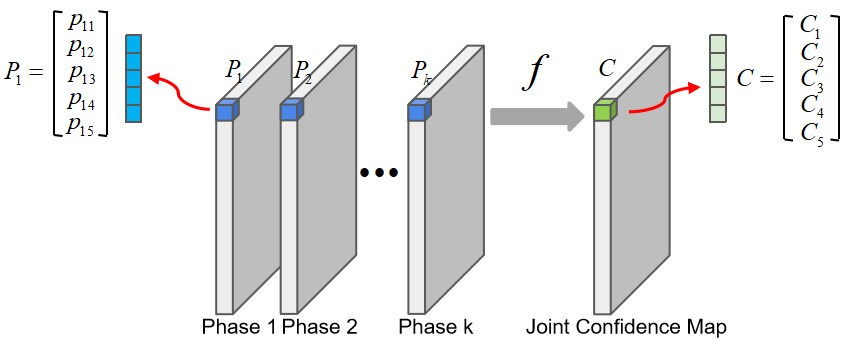
\includegraphics[width=1.0\columnwidth]{figures/images/jointConf.jpg}
		\caption{Figure placement and numbering}
	\label{fig:figure_placement}
	\end{center}
\end{figure}
In our multi-temporal training method, we abandon the previous method of explicitly measuring the unchanging region according to the distance between data domains, and use implicit prediction probability based on each classifier its own time phase. The joint confidence on multi-phases is calculated to determine pixel's category and unchanged information. The specific calculation steps of joint confidence are demonstrated here. Firstly, on each phase we train a classifier independently. After training, each classifier gives a probability prediction map $P_k$ of pixels on each phase. On each pixel of probability map, there is an array of probability whose size is the number of land cover types and the value on array represents how likely the pixel belongs to this kind of land cover type. Then we combine all the probability maps during the whole episode following the function.

\begin{equation}
    C(M_1,M_2,\dots,M_k)=\frac{(\prod\limits_{i=1}^{k}P(y_i|X_i;\theta_i))^{\frac{2}{k}}}{\frac{1}{k}\sum\limits_{i=1}^{k}P(y_i|X_i;\theta_i)}
\label{equ:conf}
\end{equation}

Here, $P_i$ denotes probability map on each single phase, $M_1,M_2,\dots,M_k$ denotes the models and $C(M_1,M_2,\dots,M_k)$ denotes the joint confidence map. In this function, we combine and reduce the category prediction information of multiple phases into a confidence map over the period of time. The goal of the function is mapping pixel's prediction probability on multi-phases to a confidence value of the whole episode. The confidence computation method is followed by the form of general harmonic mean. It has two advantages: (1) if the probabilities given by all classifiers on one pixel are greatly high, then the confidence generated will also be very high implies that it is highly likely that the pixel's type has not changed and its true type is this in this period of time ; (2) if some classifiers' probabilities are high but some are low, then the final confidence given will be determined by the gap between the low and high probability values. If the probability given by these classifiers which support the pixel's type unchanged are significantly high, then the confidence can be high possibly. And the low probability can be regarded as some special reason resulting it like seasonal change or illumination change. However, if most classifier's probabilities are very low, the final confidence must be very low suggests that the type of pixel has changed; (3) Compared with some voting methods, this mapping function provides a potential way to let these classifiers judge the pixels' type and change state.

Here, we visualize the changing map generated by the approach to show where the type has likely changed and where the type has likely unchanged.

\begin{figure}[ht!]
	\begin{center}
			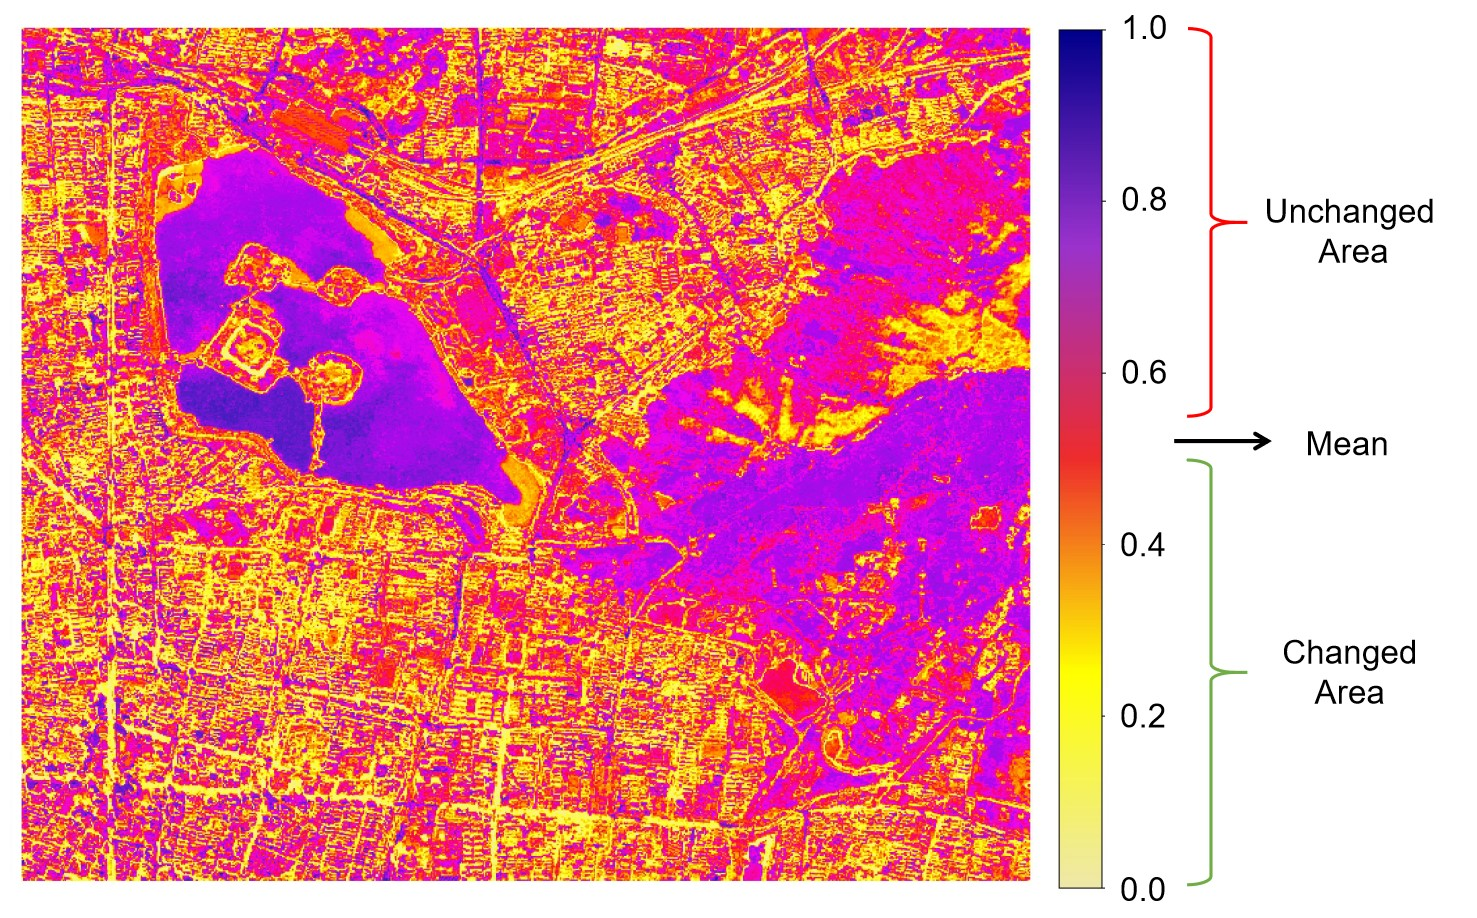
\includegraphics[width=1.0\columnwidth]{figures/images/unchangedMap.jpg}
		\caption{Figure placement and numbering}
	\label{fig:figure_placement}
	\end{center}
\end{figure}

After each round of classifiers making predictions, we can obtain a class confidence map for this period of time by using the above method, and then update the training set based on the framework of semi-supervised learning. We calculate the average confidence of one class at each round of updates, and set it as a threshold. The pixels whose confidence value of its own class of pixels is higher than this threshold will be picked, and a fixed number of samples are randomly selected to add into the training set. We repeat this process for the setting update epochs. 

\subsection{Multi-training}\label{sec:Multi-training}

\begin{algorithm}[htb] 
	\renewcommand{\algorithmicrequire}{\textbf{Input:}}
	\renewcommand{\algorithmicensure}{\textbf{Output:}}
	\caption{ Framework of Multi-training} 
	\label{alg:Framwork} 
	\begin{algorithmic}[1] 
	\REQUIRE
	The dataset of multiple phases, $D=\{D^1,\dots,D^k\}$;\\
	The set of labelled samples for each phase, $D_{l}=\{D_l^1,\dots,D_l^k\}$;\\
	The initial labelled samples number for each class, $N_l^{(0)}$;\\
	The updating unlabelled samples number for each epoch, $N_u$;\\
	The updating threshold, $\lambda$;\\
	\ENSURE
	The set of trained models, $M=\{M_1,\dots,M_k\}$;\\
	\STATE Initialize models, $M=\{M_1,\dots,M_k\}$;\\ 
	\label{code:fram:init}
	\FOR {epoch $<$ endEpochs}
	\STATE Train models on each own labelled samples;\\
	\label{code:fram:train}
	\STATE Make predictions on the whole data, generate the probability map $M_i$ for each phase; \\
	\label{code:fram:predict}
	\STATE Compute the joint confidence map with the function \ref{equ:conf};\\
	\label{code:fram:calcconf}
	\STATE Calculate the updating threshold of each class by the confidence map, $th=\lambda\times mean(\{p|p\in P_{i}, i\; denotes\;class\})$;\\
	\label{code:fram:thre}
	\STATE Randomly select the unlabelled samples whose confidence is higher than $th$ for each class with setting number $N_u$;\\
	\label{code:fram:update}
	\ENDFOR
	\RETURN $M$; 
	\end{algorithmic}
\end{algorithm}

When we perform the training according to the above algorithm, there are some details need to pay attention to, which will affect the final effect. 

\section{Study area and data}\label{sec:Study area and data}

\subsection{Study area}\label{sec:Study area}

The study area, Nanjing City, is stood in the lower reaches of the Yangtze River Plain. Located in the subtropical monsoon climate zone, it is great different in vegetation between seasons, which provides powerful support for multi-temporal training. Selected as The National Ecological Garden City, Nanjing City continues to be the first with the forest coverage rate in Jiangsu Province, which is perfect for recognition of urban green cover. So we chose Nanjing as our study area and our imagery focused on Xuanwu Lake area in the center of Nanjing. The main tree species in Nanjing City are Oriental plane, Ginkgo, Camphor and Zelkova schneideriana.

\begin{figure*}[ht!]
	\begin{center}
			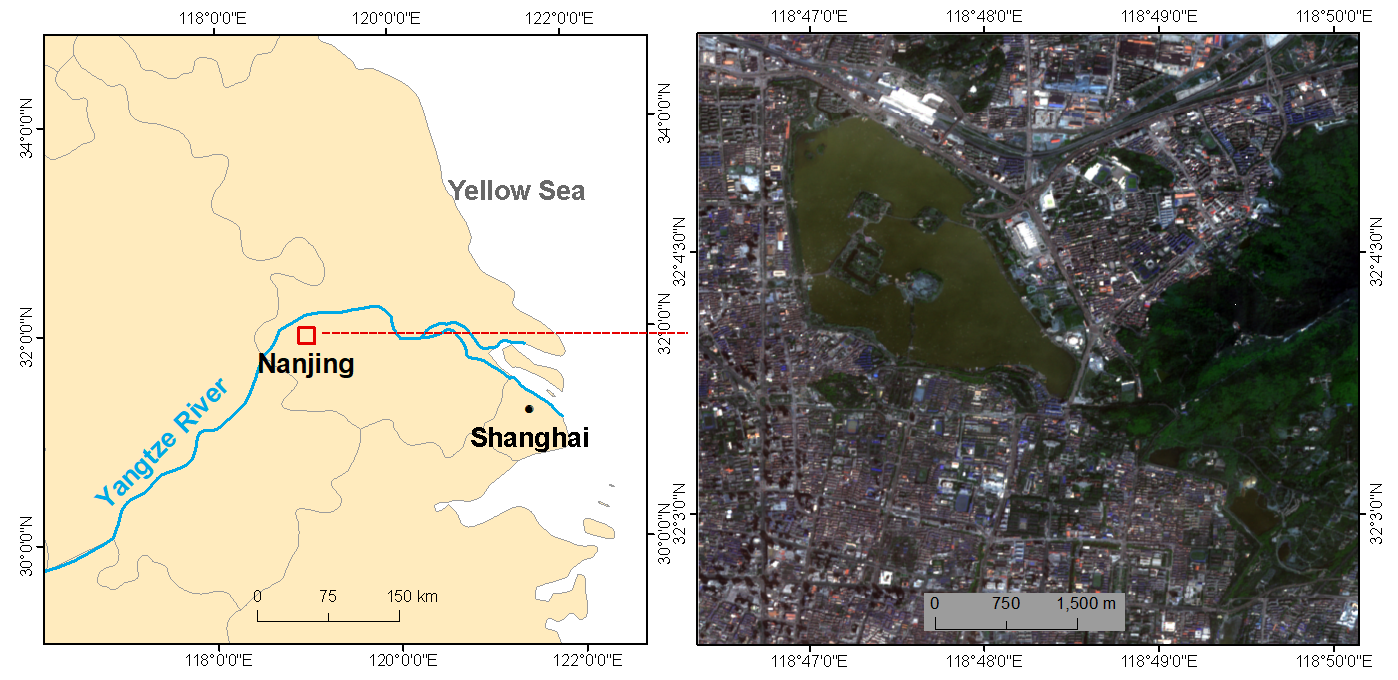
\includegraphics[width=2.0\columnwidth]{figures/images/studyArea.png}
		\caption{Figure placement and numbering}
	\label{fig:studyArea}
	\end{center}
\end{figure*}

\subsection{Data}\label{sec:Data}

This study used SENTINEL-2-MSI images of Xuanwu Lake area in Nanjing, as shown in Fig.\ref{fig:studyArea}. The images contains $772\times653$ pixels, and each has four bands with a spatial resolution of 8.98 m. Four bands are Blue(0.46~0.52$\mu m$), Green(0.54~0.58$\mu m$), Red(0.50~0.80$\mu m$), NIR(0.78~0.90$\mu m$). Sentinel-2 is a wide-swath, high-resolution, multi-spectral imaging mission supporting Copernicus Land Monitoring studies, including the monitoring of vegetation, soil water cover, as well as observation of inland waterways and coastal areas.
We selected multiple images from August 15,2016 to June 30,2020, every three months. All images are preprocessed to eliminate cloud interference. The three-month sampling interval ensures the difference of the vegetation, while the images of the same month between years ensure the similarity of the vegetation. Through these operations, we obtained varied multi-temporal imagery in Nanjing. 
In order to augment our existing data, we try to construct some meaningful indices on the basis of previous researches. The following nine indices are chosen: 

\begin{enumerate}
	\item NDVI
	\begin{equation}
		NDVI=\frac{nir-red}{nir+red}
	\end{equation}
	This index takes advantage of the contrast of the characteristics of two bands from a multispectral raster dataset—the chlorophyll pigment absorptions in the red band and the high reflectivity of plant materials in the near-infrared (NIR) band.
	\item NDWI
	\begin{equation}
		NDWI=\frac{green-nir}{green+nir}
	\end{equation}
	This is an index for delineating and monitoring content changes in surface water. It is computed with the near-infrared (NIR) and green bands.
	\item CIg
	\begin{equation}
		CIg=\frac{nir}{green}-1
	\end{equation}
	This is a vegetation index for estimating the chlorophyll content in leaves using the ratio of reflectivity in the near-infrared (NIR) and green bands. 
	\item EVI
	\begin{equation}
		EVI=\frac{2.5(nir-red)}{nir+6red-7.5blue+1}
	\end{equation}
	This is an optimized vegetation index that accounts for atmospheric influences and vegetation background signal. It's similar to NDVI but is less sensitive to background and atmospheric noise, and it does not become as saturated as NDVI when viewing areas with very dense green vegetation. 
	\item GNDVI
	\begin{equation}
		GNDVI=\frac{nir-green}{nir+green}
	\end{equation}
	This is a vegetation index for estimating photo synthetic activity and is a commonly used vegetation index to determine water and nitrogen uptake into the plant canopy. 
	\item MTVI
	\begin{equation}
		MTVI=\frac{1.5(1.2(nir-green)-2.5(red-green))}{\sqrt{(2nir+1)^2-(6nir-5\sqrt{red})-0.5}}
	\end{equation}
	This is an index computed with previous temporal NDVI and latter temporal NDVI.
	\item SAVI
	\begin{equation}
		SAVI=\frac{nir-red}{nir+red+L}(L+1)
	\end{equation}
	This is a vegetation index that attempts to minimize soil brightness influences using a soil-brightness correction factor. This is often used in arid regions where vegetative cover is low.
	\item MSAVI
	\begin{equation}
		MSAVI=0.5(2(nir+1)-\sqrt{(2nir+1)^2-8(nir-red)})
	\end{equation}
	This index tries to minimize the effect of bare soil on the SAVI. 
	\item VARI
	\begin{equation}
		VARI=\frac{green-red}{green+red-blue}
	\end{equation}
	This is a vegetation index for estimating vegetation fraction quantitatively with only the visible range of the spectrum.
\end{enumerate}

We sample from the data and calculate the correlation degree between the feature and the ground category. In the following figure, we show the correlation degree of these indicators. The first five indices (NDVI, MSAVI, MTVI, SAVI, VARI) and the original four bands are combined to form 9 dimensional features, which are the final features of the data set.

\begin{figure}[ht!]
	\begin{center}
			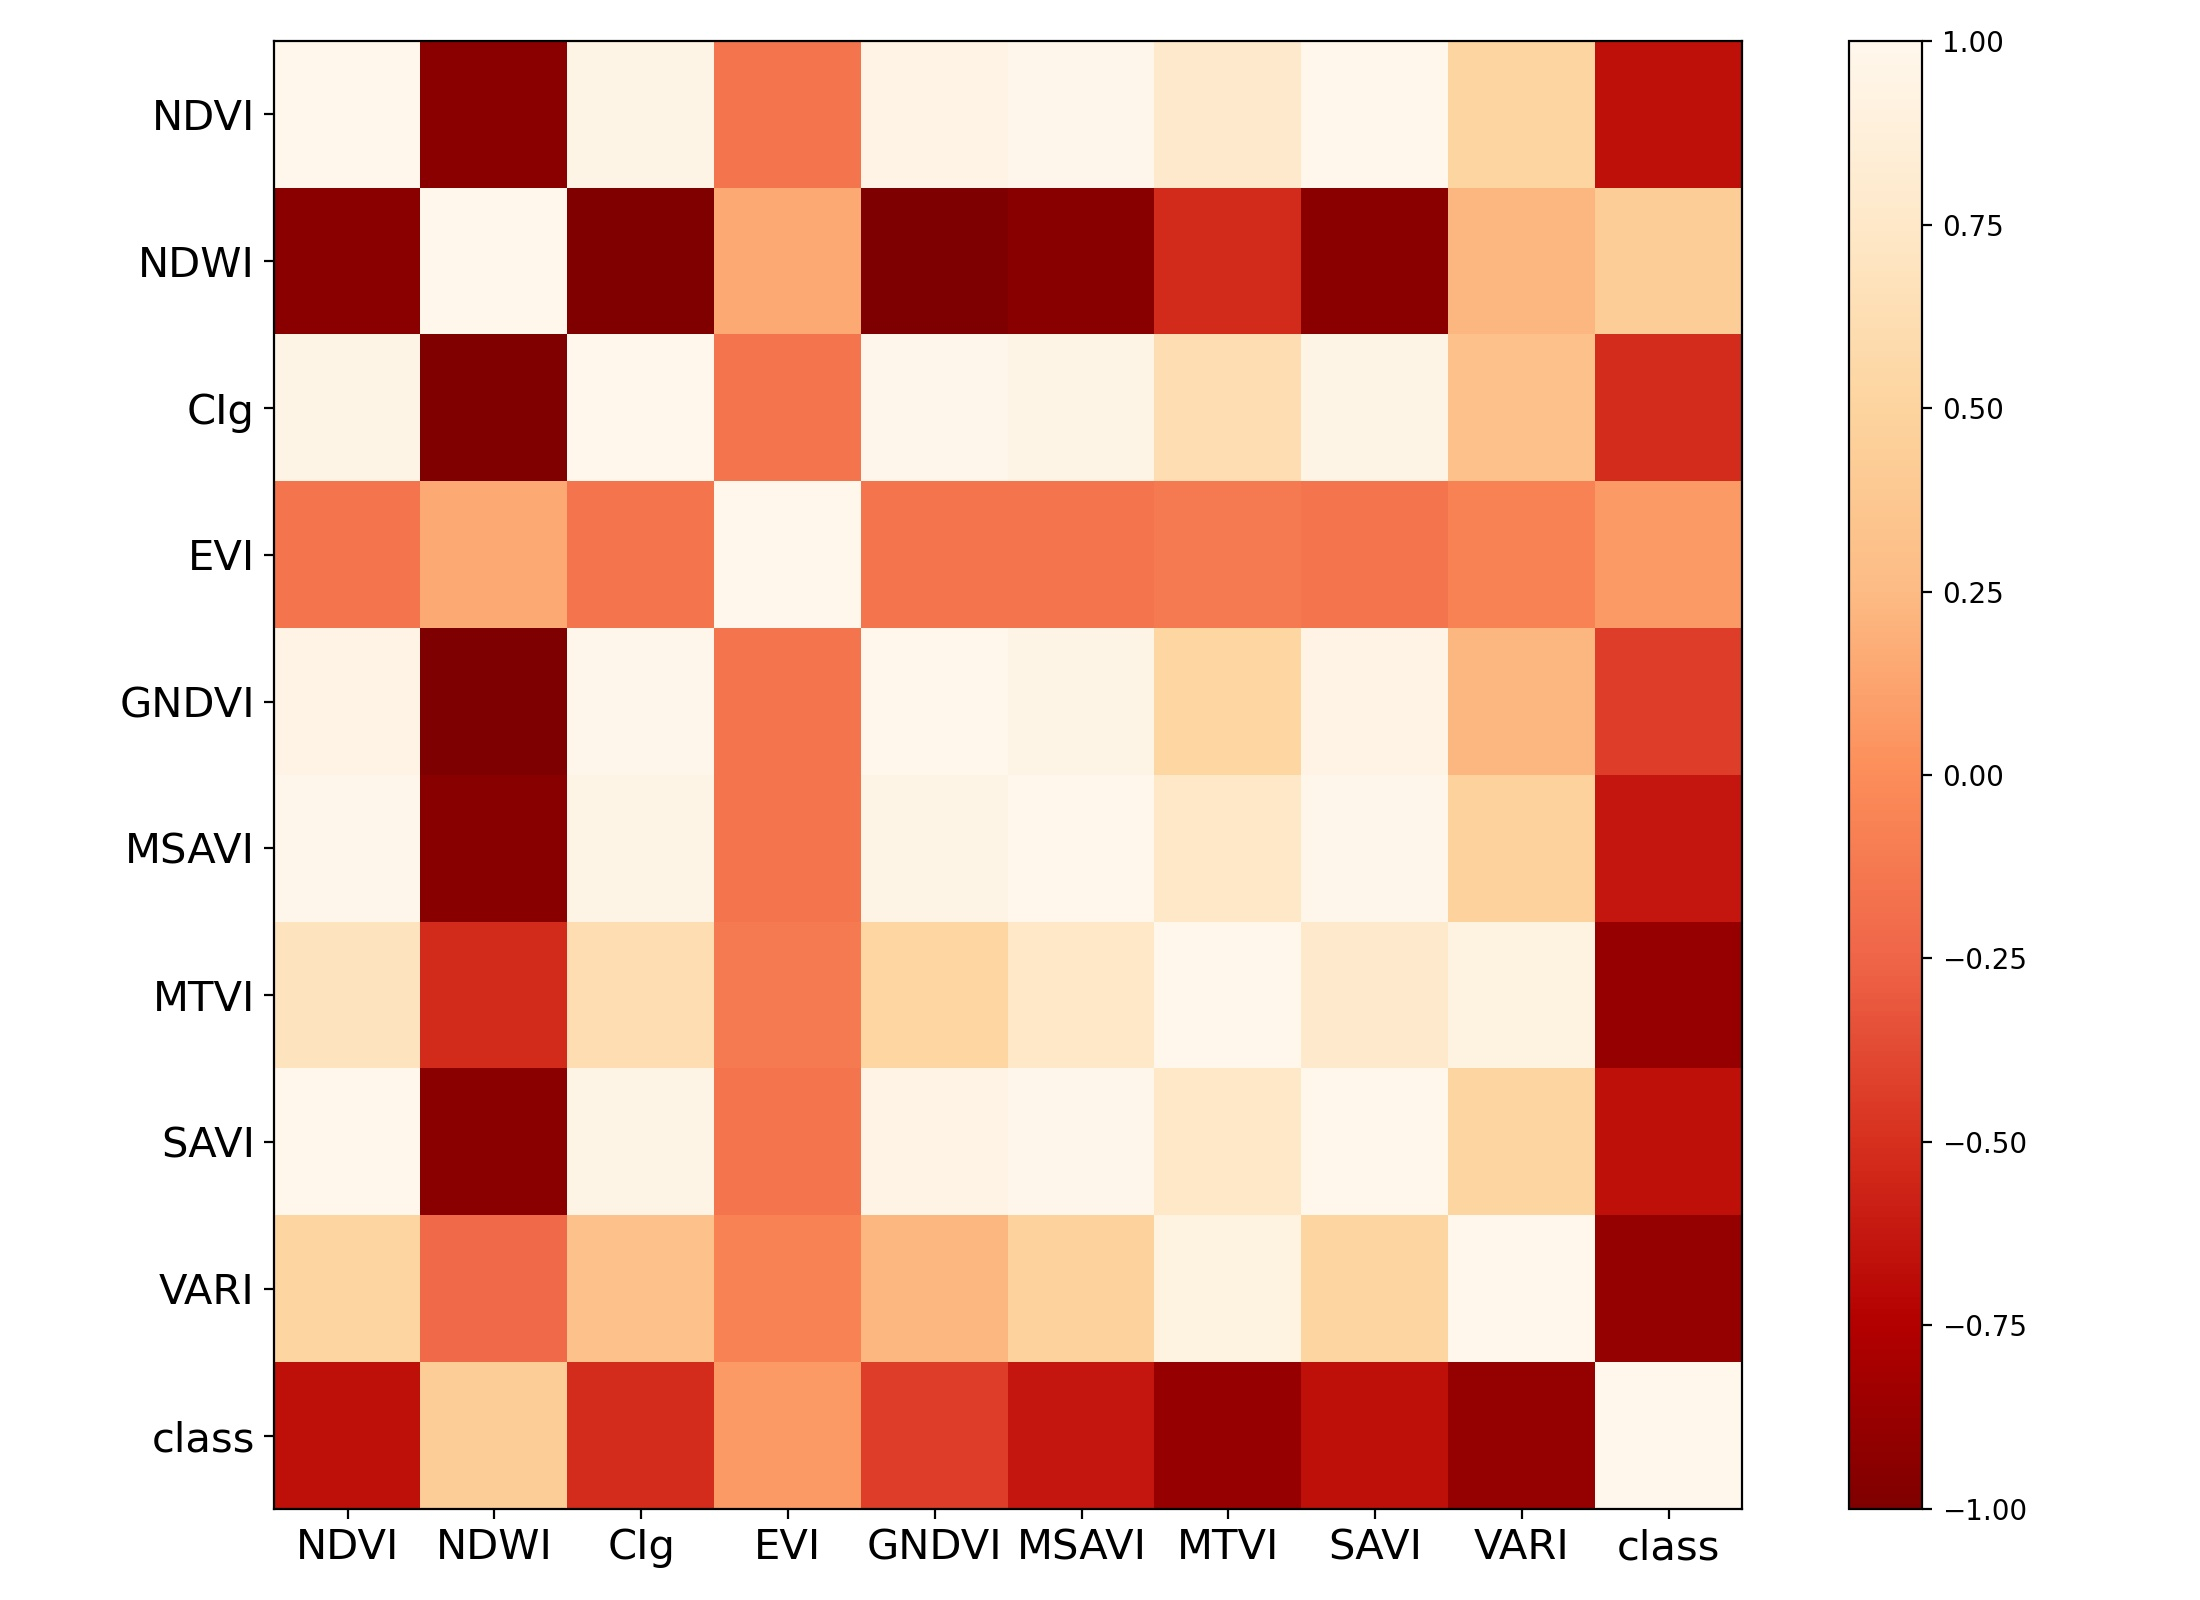
\includegraphics[width=1.0\columnwidth]{figures/images/corr.jpg}
		\caption{Figure placement and numbering}
	\label{fig:studyArea}
	\end{center}
\end{figure}
On each phase, we randomly marked the same number of samples on image and the number of  each class labeled are 1,000. We further divide the labeled data set into training set and testing set according to 1:4 ratio. More precisely, the training set here should be named training pool for the reason that subsequent training samples are selected from it with a fixed size independently and repeatedly to form the final training set during the experiment.

\begin{table}[ht!]
	\begin{center}
		\begin{tabular}{c|c|c}
		\toprule
		Class & Training set & Validation set  \\
		\midrule
		Vegetation           & 200 & 800\\
		Shadow               & 200 & 800\\
		Water                & 200 & 800\\
		Road                 & 200 & 800\\
		Building             & 200 & 800\\
		\midrule
		Total                & 1000 & 4000\\
		\bottomrule
		\end{tabular}
	\caption{}
	\end{center}
\end{table}

\section{Experimental design}\label{sec:Experimental design}

\subsection{Validation metric}

In our experiments, F1-score is selected as the validation metric which is defined in for its advantages that it requires both recall and precision high. They are all expressed through the calculated TP (True Positives), FP (False Positives) and FN (False Negatives). If we have a class l, then TP is the number of pixels that have been correctly classified as l. FP is the number of pixels that have been wrongly classified as l. Finally, FN represents the pixels that belong to l but the model has associated them to some other class. 
\begin{equation}
	P=\frac{TP}{TP+FP}
\end{equation}
\begin{equation}
	R=\frac{TP}{TP+FN}
\end{equation}
\begin{equation}
	F1=\frac{2PR}{P+R}
\end{equation}

\subsection{Experimental setup}

Two kinds of experiments were designed to evaluate the performance of multi-training as well as the effect of unlabeled samples’ selection and multiple temporal combination. F1-score is used to represent the advantages and disadvantages of the model, and the average value and variance under multiple independent repeated experiments to reflect the accuracy and stability of the model under different time phases and parameter combinations. In our experiments, some necessary parameters and their explanations are listed in the table.

\begin{table}[ht!]
	\begin{center}
		\begin{tabular}{c|p{0.7\columnwidth}}
		\toprule
		Parameter & Meaning  \\
		\midrule
		$N_t$ & Number of phases combined\\
		$N_l$ & Number of labeled samples for each class initially\\
		$N_u$ & Number of updating unlabeled samples for each class each epoch\\
		$\sigma$ & Trade-off to balance the difference and the confidence\\
		$N_{iter}$ & Number of iterations of multi-training\\
		$N_{est}$ & Number of estimator of each base classifier\\
		\bottomrule
		\end{tabular}
	\caption{}
	\end{center}
\end{table}

(a)In order to explore the influence of the combination of time phase on the algorithm and decide the best phase combination method, we adjust the number of time phase to test the improved accuracy of the algorithm for small sample training sets on multi-temporal remote sensing images. In our experiment, the number of time phases is {3, 4, 5, 6, 7, 8}, and images started from 2017. The average improved accuracy under multiple time phases is set as the final measurement. Because other methods are not directly related to the number of time phases, only our method in this paper is discussed at this part.

(b)In the second experiment, we start to compare average accuracy and standard deviation between different methods on this task. The second experiment contains three sub-experiments which are designed to evaluate the number of labeled and unlabeled samples and the confidence threshold’s effect to the model’s accuracy. To achieve this goal, we change the number of labeled samples for each class before training and the number of unlabeled samples when updating the training set and adjust the threshold of confidence when selecting the unlabeled samples. In out experiment, $N_l$ ranges from 1 to 19 with step 2, $N_u$ varies from 5 to 50 with step 5. 
Here we represent the experiments’ name and parameters setting in each experiment.

\begin{table}[ht!]
	\begin{center}
		\begin{tabular}{c|cccc}
		\toprule
		Name & $N_l$ & $N_u$ & $N_t$ &$\sigma$ \\
		\midrule
		Selection of parameter $N_t$ & 1:2:3 & 5:5:10 & 3:1:8& 1.0\\
		Selection of parameter $N_l$ & 1:2:19& 5:5:10 & 4& 1.0\\
		Selection of parameter $N_u$ & 1:2:3& 5:5:50 & 4& 1.0\\
		\bottomrule
		\end{tabular}
	\caption{}
	\end{center}
\end{table}

\section{Results}\label{sec:Results}

\subsection{classification results of Multi-training}

In order to represent the results of vegetation extraction intuitively and analyze qualitatively, we compared the classification results under four phases and highlighted the area of vegetation extraction. In order to facilitate positioning, we also visualize the Xuanwu Lake in the result maps. The images on the left of the figure below is the study area of Sentinal image under four phases, the middle is the vegetation result map extracted by our algorithm, and the right column is the vegetation extraction result obtained by semi-supervised learning method of the single phase. From the comparison of results given by our algorithm and single-phase, we can see that the vegetation extracted by our algorithm is more delicate and accurate. Although based on the classification of pixels, the results of our extraction are still very consistent in the area with wide coverage of vegetation. In contrast, the vegetation area extracted by single-phase semi-supervised learning method is relatively broken. In the identification of vegetation cover in urban blocks, we can clearly find that most of the vegetation is distributed along the road in our result maps. The vegetation extracted by our algorithm has better consistency during this period and can reflect the influence of phase change on vegetation, such as the decrease and increase of mountain vegetation caused by seasonal change. Compared with the training results under large-scale labeled samples, our algorithm can even achieve similar classification results. Our multi-training algorithm has a significant advantage in mutli-temporal vegetation extraction.

\begin{figure*}[ht!]
	\begin{center}
			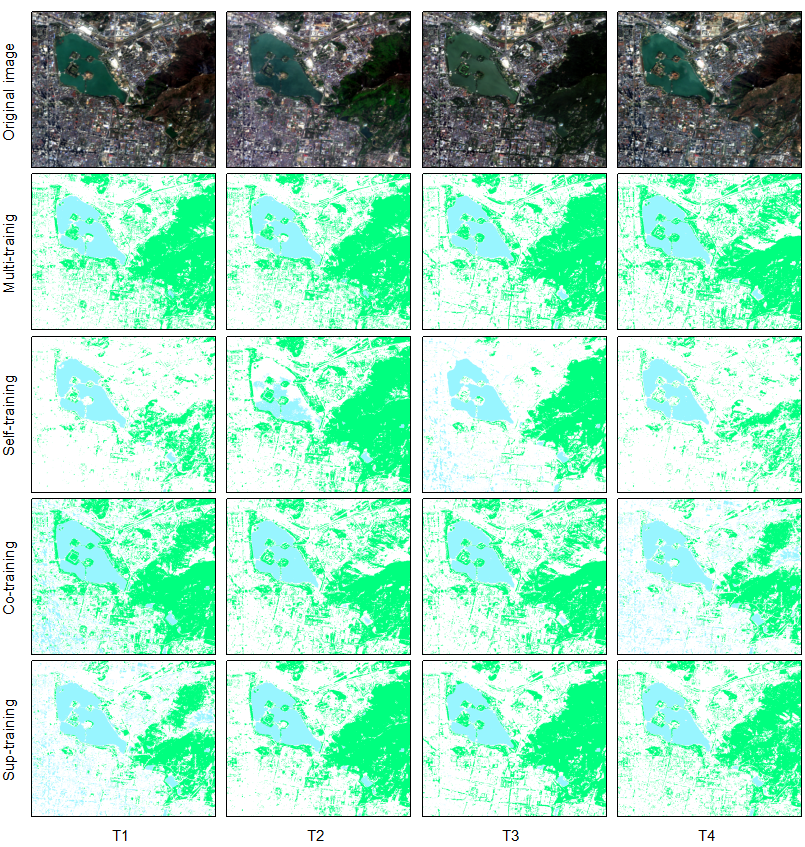
\includegraphics[width=2.0\columnwidth]{figures/images/resultMap2.png}
		\caption{Figure placement and numbering}
	\label{fig:studyArea}
	\end{center}
\end{figure*}

\subsection{Updating process during Multi-training}

\begin{figure*}[ht!]
	\begin{center}
			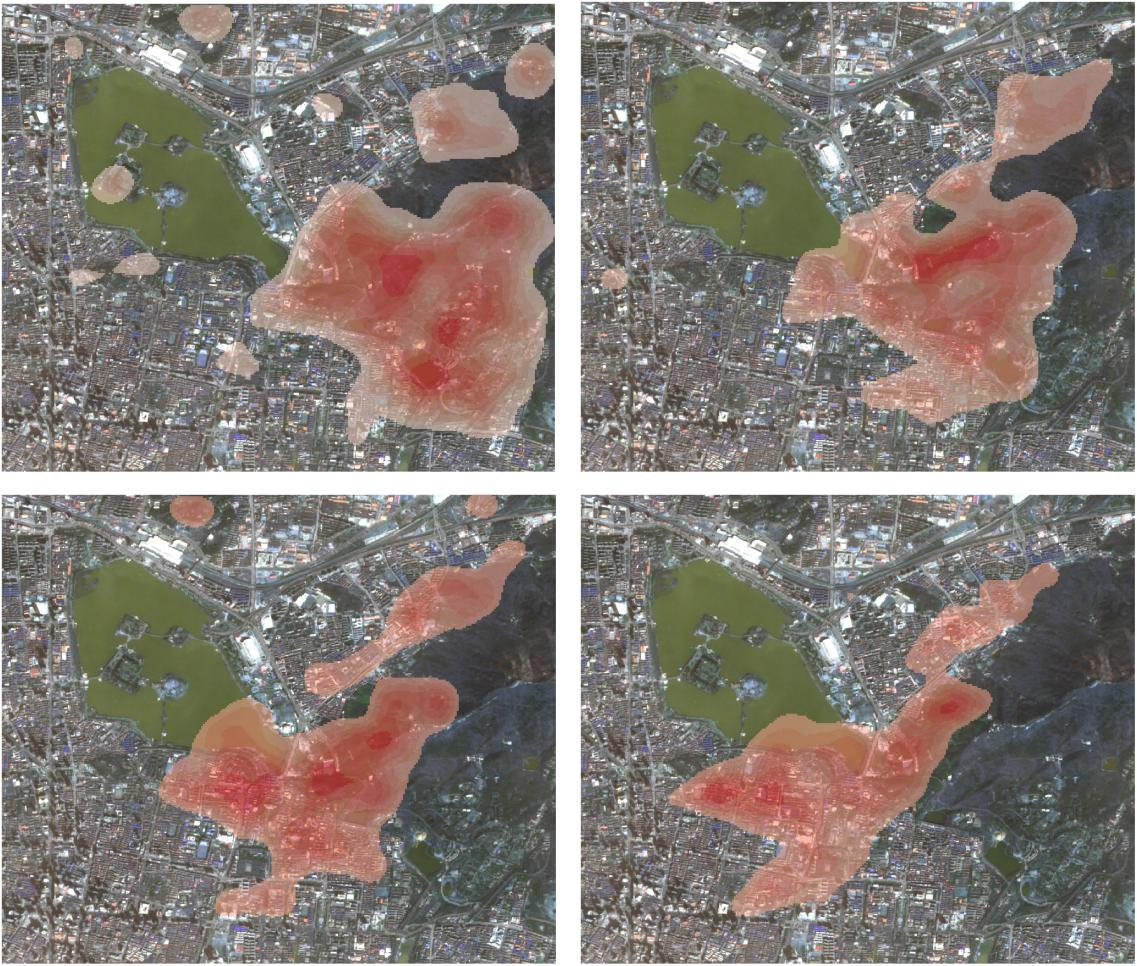
\includegraphics[width=2.0\columnwidth]{figures/images/update_loc.jpg}
		\caption{Figure placement and numbering}
	\label{fig:updateloc}
	\end{center}
\end{figure*}

In Fig.\ref{fig:updateloc}, the unlabeled points derived by iterations is shown. Nl is 1 and Nu is 5. In the (a), we can see that in the beginning the points selected are generally from the woodland or places beside the water, which is typical vegetation areas. With the increase of the number of iterations, the ability of the classifier is improved, and the selection area extend to building area in the lower left part of the image. In building area, the vegetation are only the street trees and some lawn, the classifier still selects them out, which shows the power of the classifier. However, few unlabeled points are selected from the water area in (d). Wrong sample selection is inevitable in the process of enlarging sample size. The proportion of the wrong selection is quite low, and a small number of wrong samples do not affect the model actually. In addition, the final result graph has shown that the water area and vegetation are well distinguished. The classifier has the ability to tolerate the wrong samples.

\subsection{Performance of Multi-training}

\begin{table*}[ht!]
	\begin{center}
	\resizebox{\textwidth}{!}   & 0.820    & 0.833  & 1.6\%          & 0.822     & 0.831    & 1.1\%  & 0.953 & 0.982 & 2.8\%\\
	Shadow               & 0.690    & 0.799  & \textbf{15.8\%}   & 0.676    & 0.724  & 7.1\%         & 0.690     & 0.718    & 4.0\%  &0.912 &0.965 & 5.3\% \\
	Water                & 0.807    & 0.832  & 3.0\%   & 0.779    & 0.837  & \textbf{7.5\%}         & 0.790     & 0.814    & 3.0\%   & 0.929 & 0.979 & 5.0\%\\
	Road                 & 0.645    & 0.691  & 7.1\%   & 0.624    & 0.625  & 0.1\%         & 0.628     & 0.603    & -4.0\%  & 0.786 & 0.902 & \textbf{11.5\%} \\
	Building             & 0.466    & 0.531  & 13.9\%  & 0.421    & 0.468  & 11.2\%          & 0.417     & 0.448    & 7.3\%  &0.715 &0.889 &\textbf{17.3\%} \\
	\midrule
	Ave.                 & 0.688    & 0.753  & \textbf{9.5\%}   & 0.664    & 0.698  & 5.0\%         & 0.670     & 0.683    & 2.0\%  &0.859 & 0.943 &8.4\% \\
	\bottomrule
	\end{tabular}
	}
	\caption{Performances of multi-training, co-training and self-training (labeled data size=1,unlabeled data size=15)}
	\end{center}
\end{table*}
To further illustrate the effectiveness of the multi-training, we compared this proposed classification method with several classification methods by classifying all four datasets. More specifically, we compared the multi-training with self-learning, co-training(Zhu, 2016) and super-training.

The self-training is mentioned before in 5.1 which is semi-supervised learning method of the single phase. The co-training is a semi-supervised classification method. And the super-training is supervised classification method which used fifth numbers of Nl and Nu than semi-supervised methods. The F1-score of vegetation of four method is shown as Fig.7. (a) set Nu equaling 5 and (b) set Nu equaling 10. In the phases of 02.11 and 12.18, the multi-training get a obvious higher F1-score than other three methods. By changing of the time phase, the precise of classification from the other three methods showed the unstability, while the multi-training still got a generally satisfactory classification result. This verified the robustness  of the multi-training. 

From (a) to (b), which increased Nu from 5 to 10, the F1-score of multi-training, self-training and co-training has improved. This indicates that the unlabeled samples can help represent the general classification problem with fewer labeled samples. On the contrary, the F1-score of super-training didn’t improve roughly. Because the super-training has already used much more numbers of Nl and Nu than three semi-supervised methods. The little increasing of Nu will not improve the performance well. And in the next section, we will discuss the influence of Nl in detail.

The the initial and final F1-score of five objects are shown In the Fig.8. The final F1-score represent the precise of the three semi-supervised classifier after several iterations. Nl is are chosen 1. The initial F1- score of vegetation of the three methods are nearly the same. Because they have the same operation before the chosen of the unlabeled samples. After the chosen of the unlabeled samples and several iterations, the F1-score of the vegetation of the multi-training has improved rapidly, while other two methods merely have little improvement. This indicates our method of the selection of unlabeled sample has a great advantage. For multi-training method, not only the F1-score of vegetation, but also the shadow, road, building and overall F1-socre have a great improvement. This shows that the multi-training method has general applicability. And it is likely to use this method in extraction of other objects.

\subsection{Influence of unlabeled sample selection}

\begin{figure*}[ht!]
	\centering
	
	\subfigure[pic1.]{
		\centering
		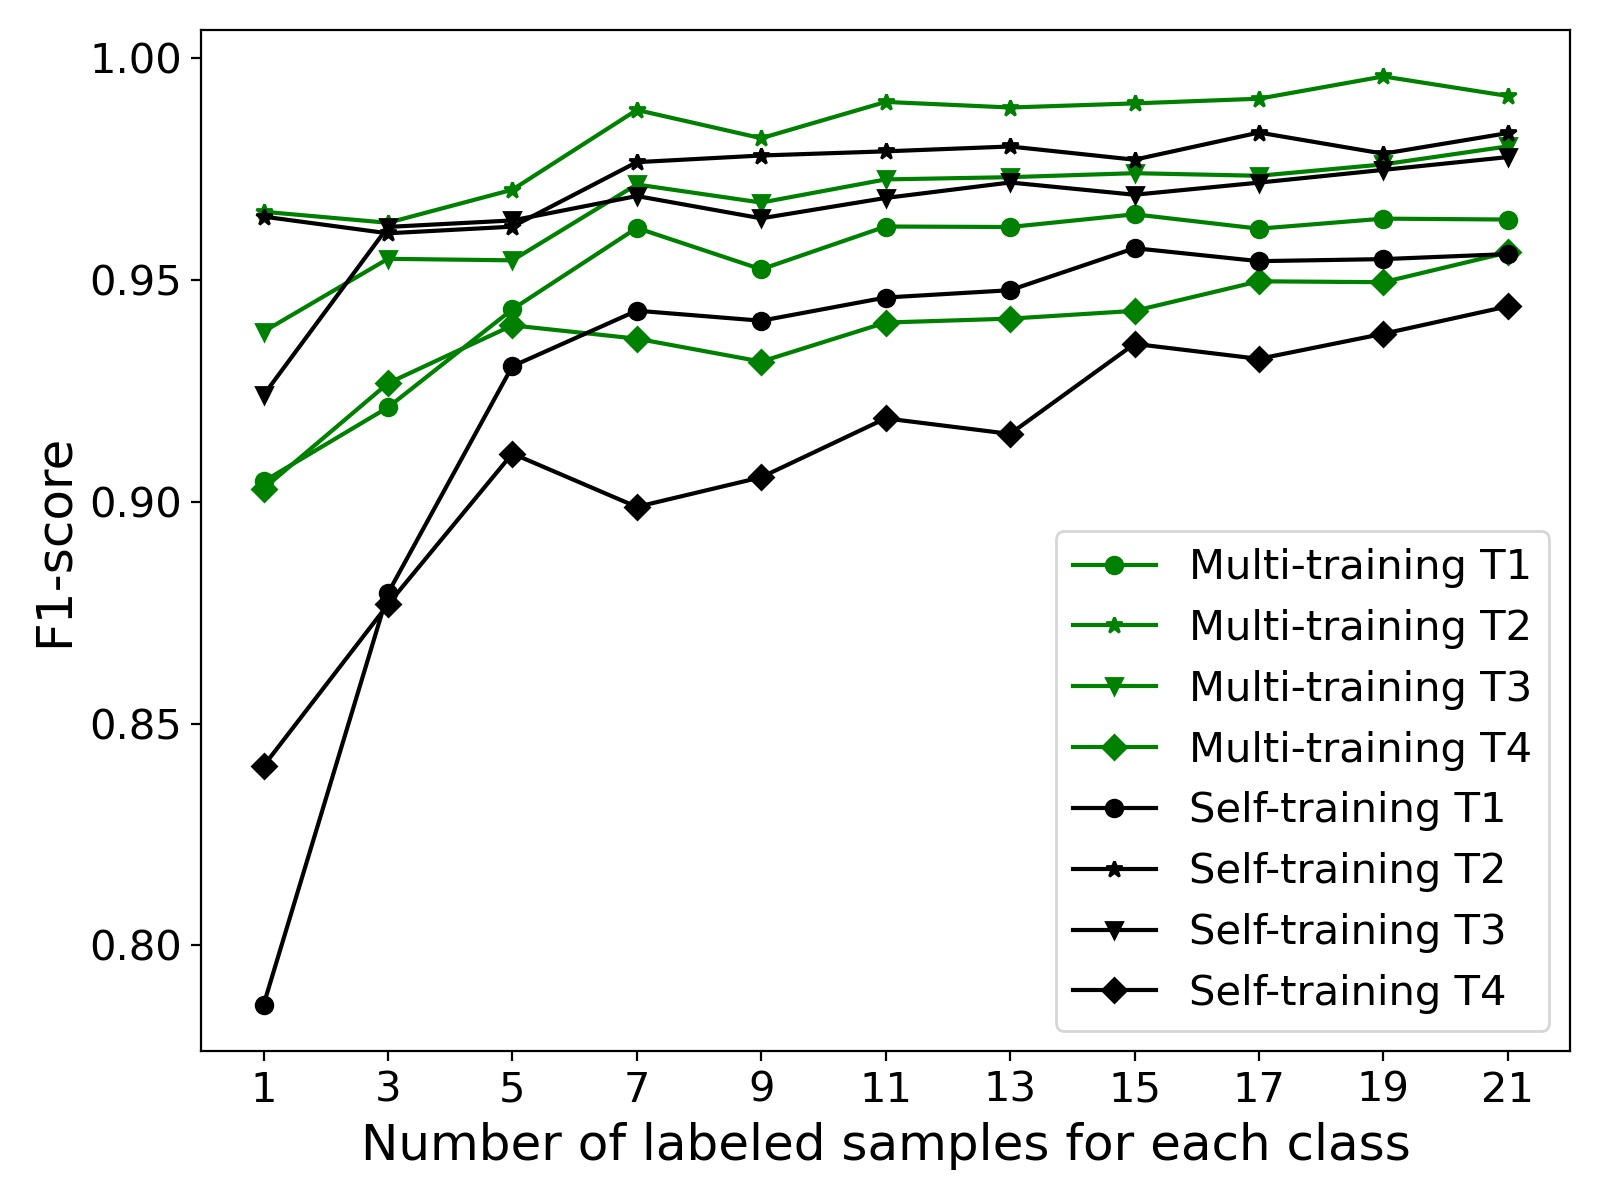
\includegraphics[width=0.5\columnwidth]{figures/images/multi_self_veg_unlabel5_final_trend_mean.jpg}
		%\caption{fig1}
	}%
	\subfigure[pic2.]{
		\centering
		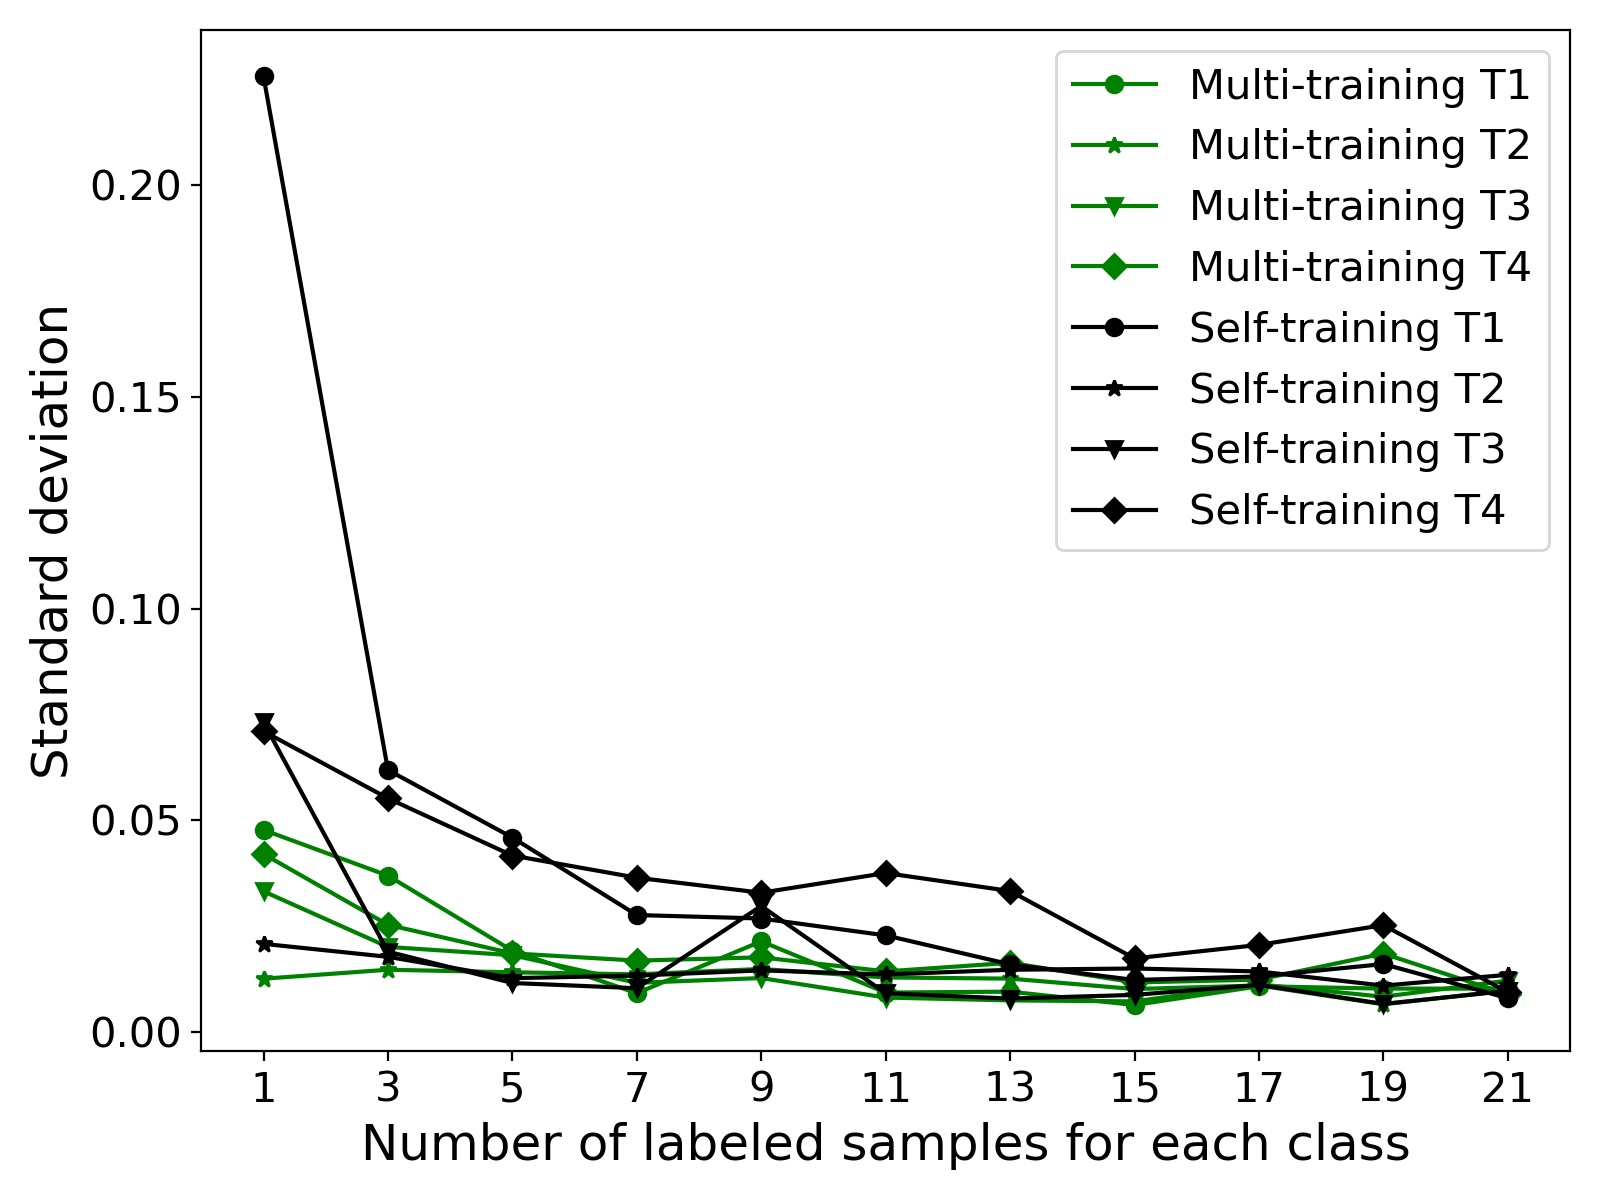
\includegraphics[width=0.5\columnwidth]{figures/images/multi_self_veg_unlabel5_final_trend_std.jpg}
		%\caption{fig2}
	}%
	\subfigure[pic2.]{
		\centering
		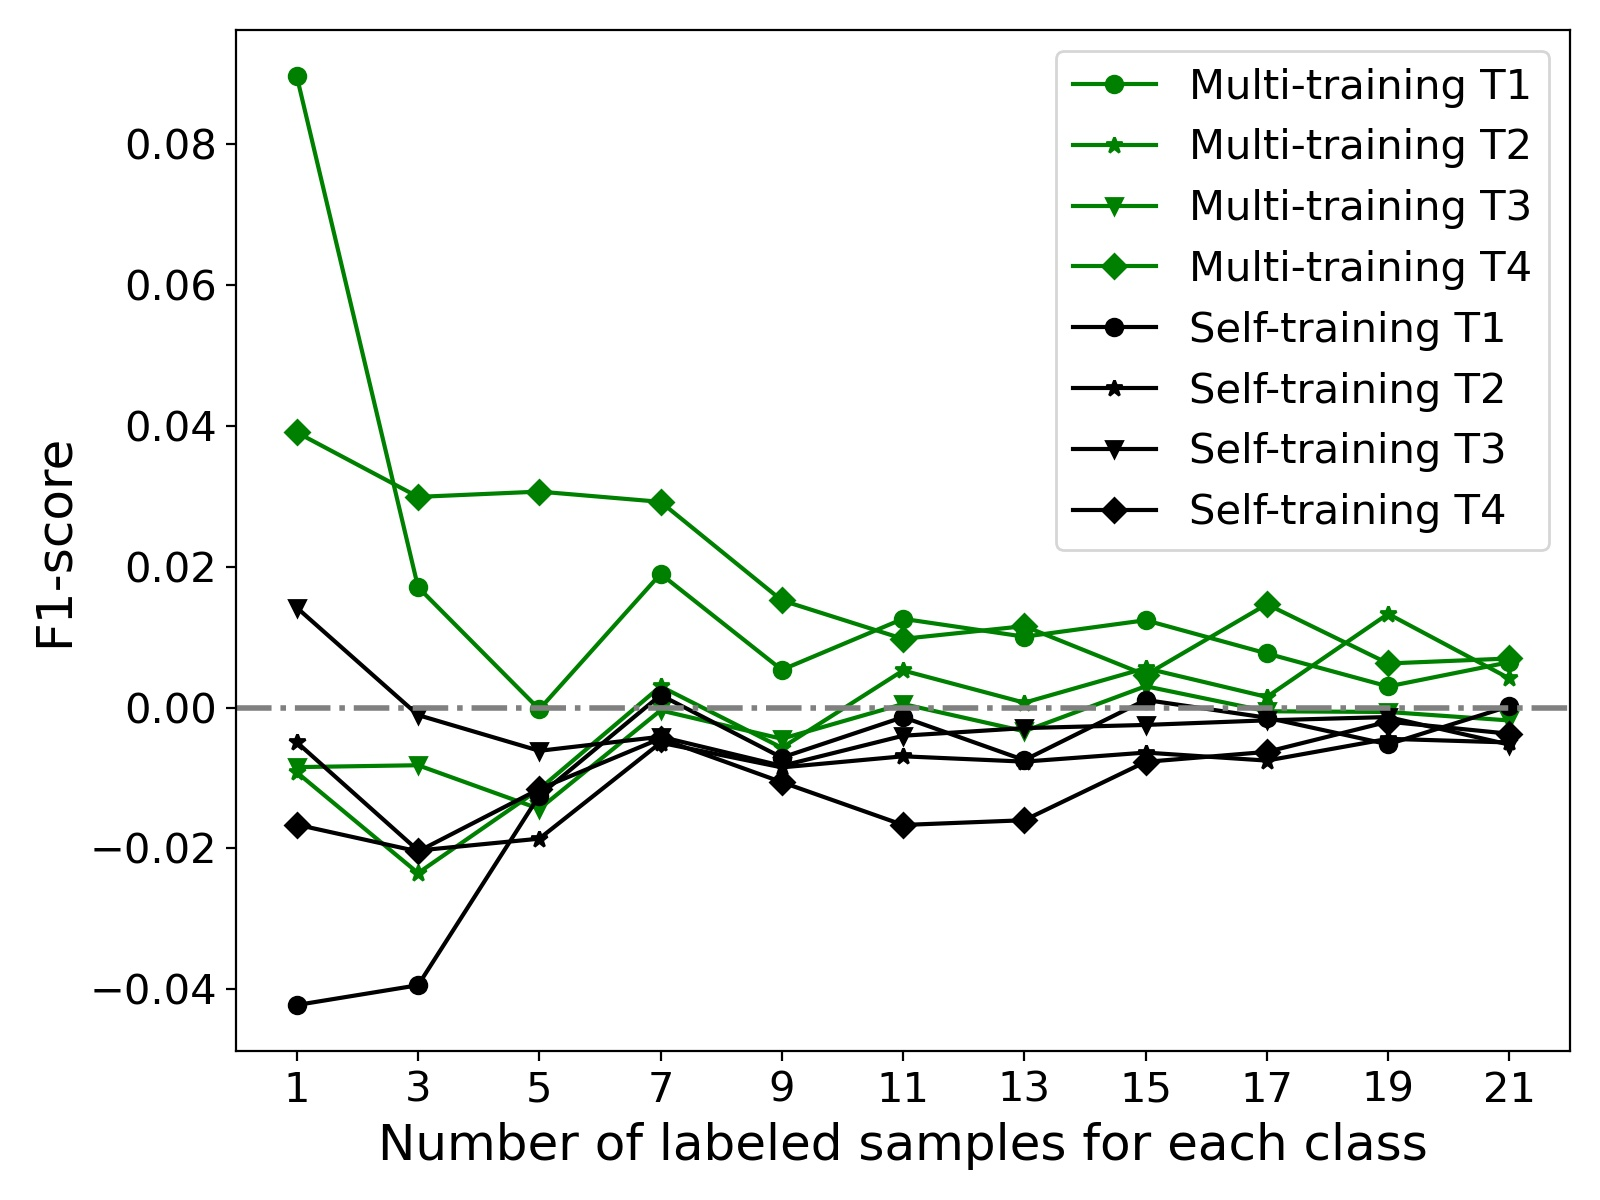
\includegraphics[width=0.5\columnwidth]{figures/images/multi_self_veg_unlabel5_improved_trend_mean.jpg}
		%\caption{fig2}
	}%
	\subfigure[pic2.]{
		\centering
		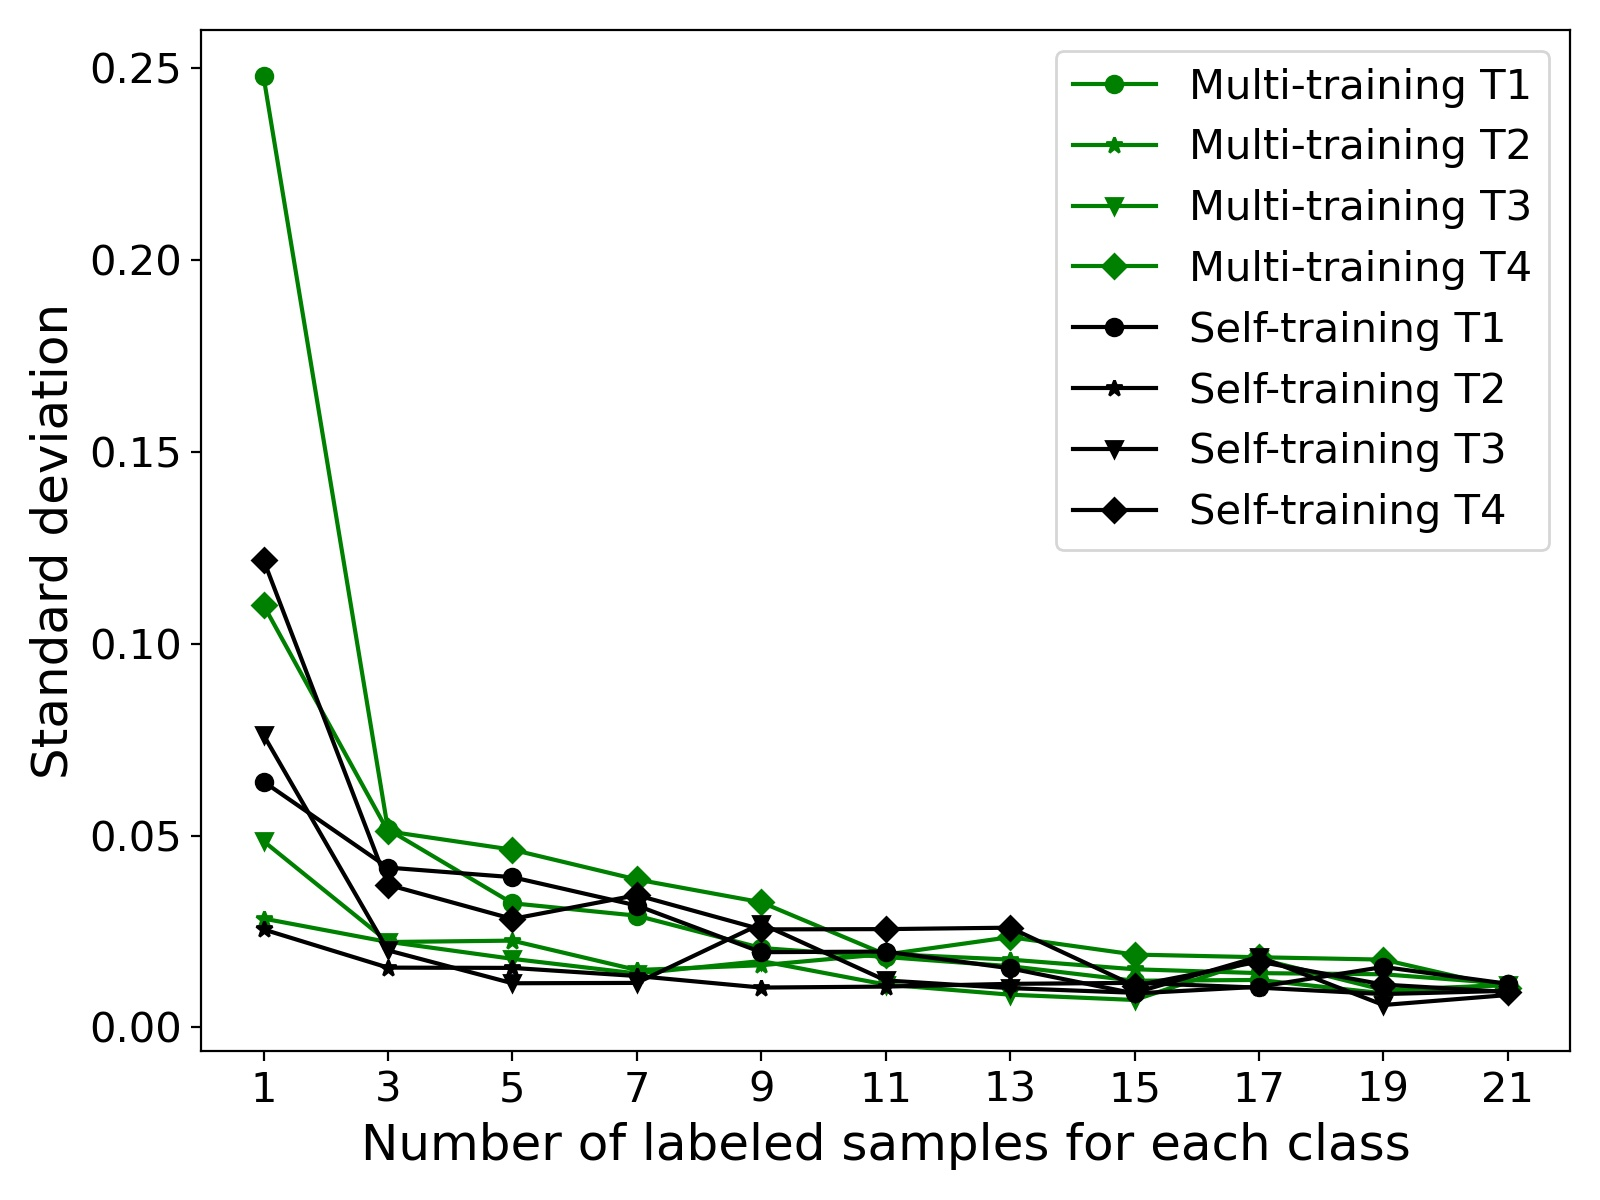
\includegraphics[width=0.5\columnwidth]{figures/images/multi_self_veg_unlabel5_improved_trend_std.jpg}
		%\caption{fig2}
	}%
	\quad
	\subfigure[pic3.]{
		\centering
		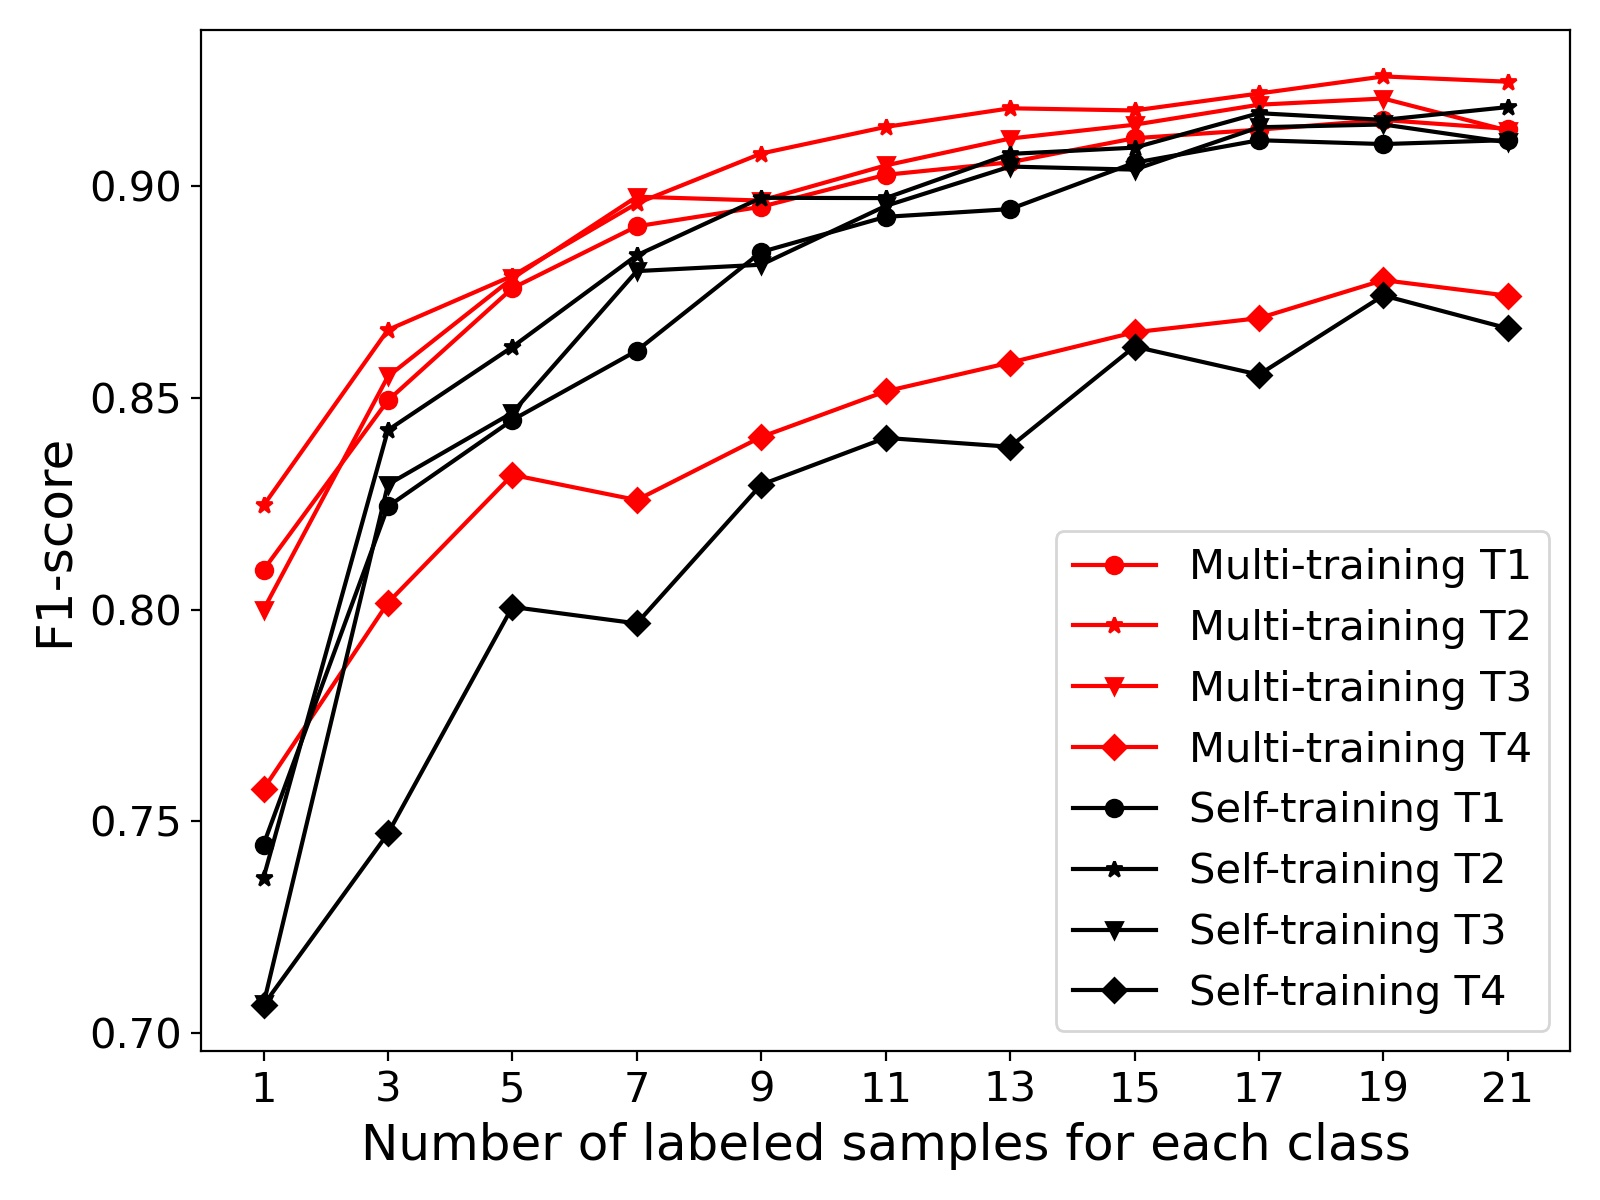
\includegraphics[width=0.5\columnwidth]{figures/images/multi_self_total_unlabel5_final_trend_mean.jpg}
		%\caption{fig2}
	}%
	\subfigure[pic4.]{
		\centering
		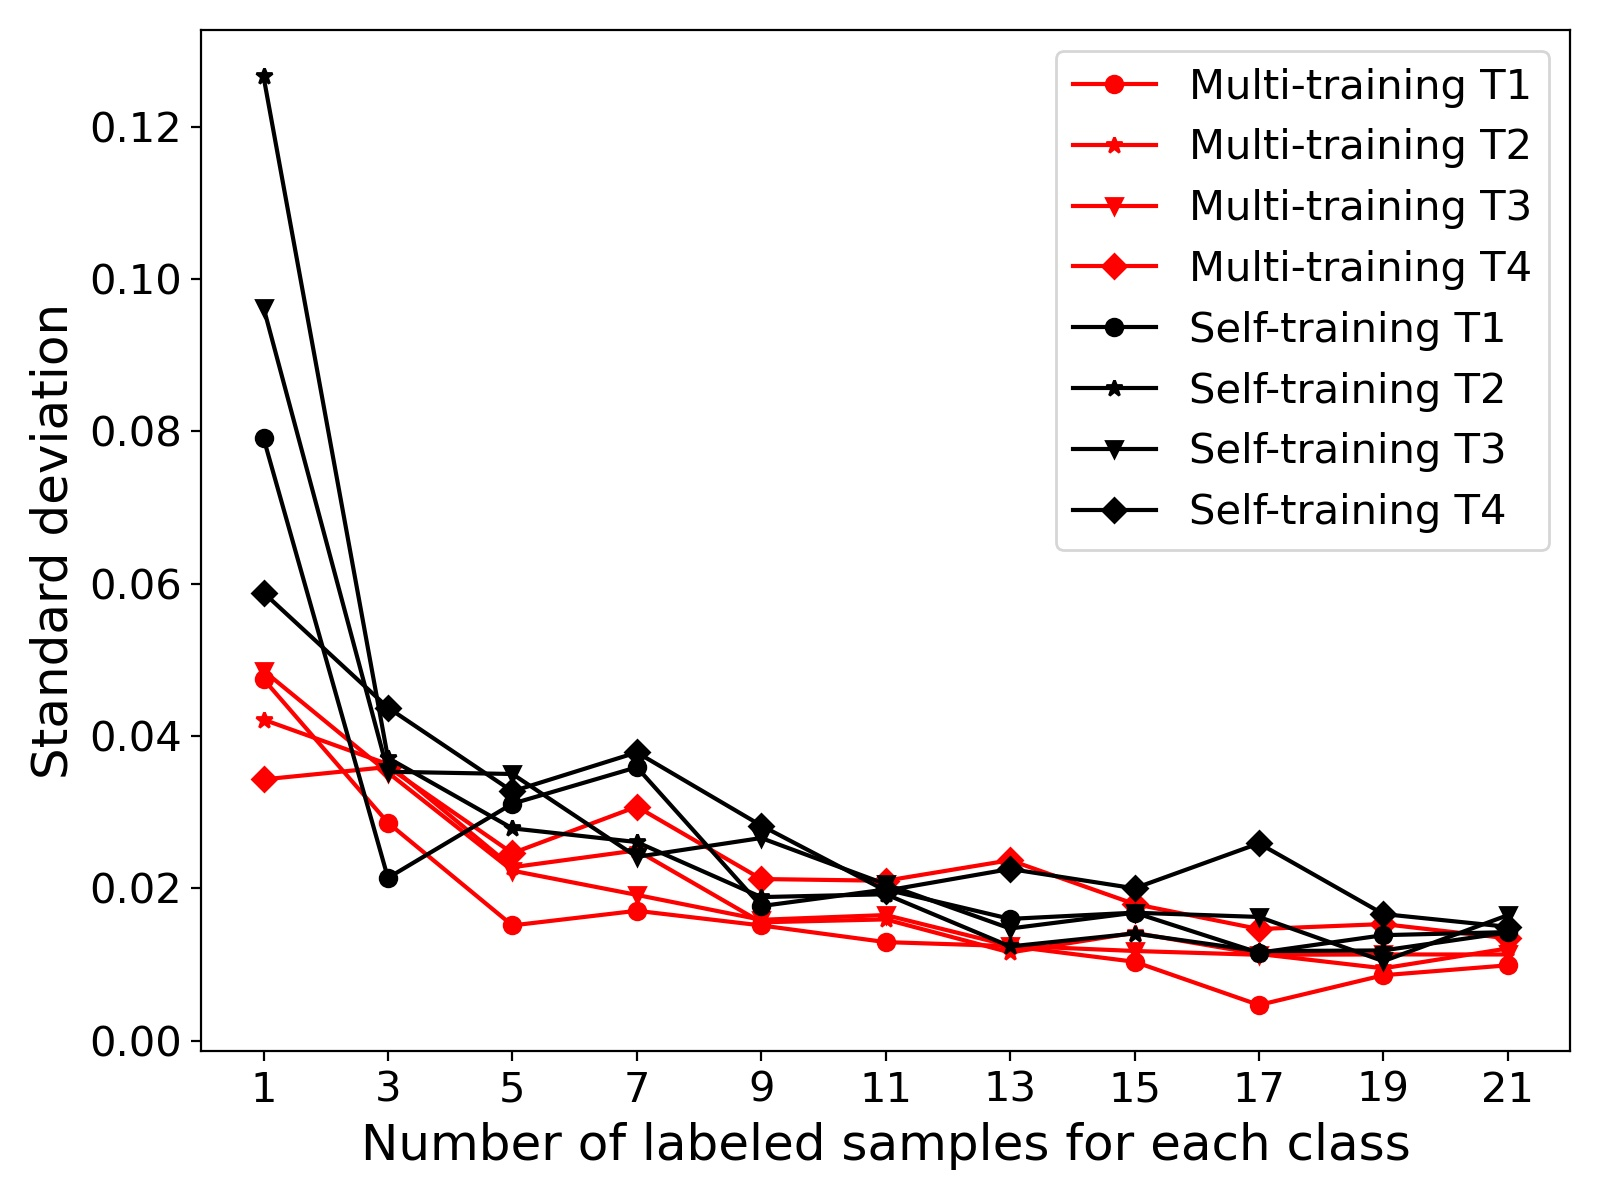
\includegraphics[width=0.5\columnwidth]{figures/images/multi_self_total_unlabel5_final_trend_std.jpg}
		%\caption{fig2}
	}%
	\subfigure[pic2.]{
		\centering
		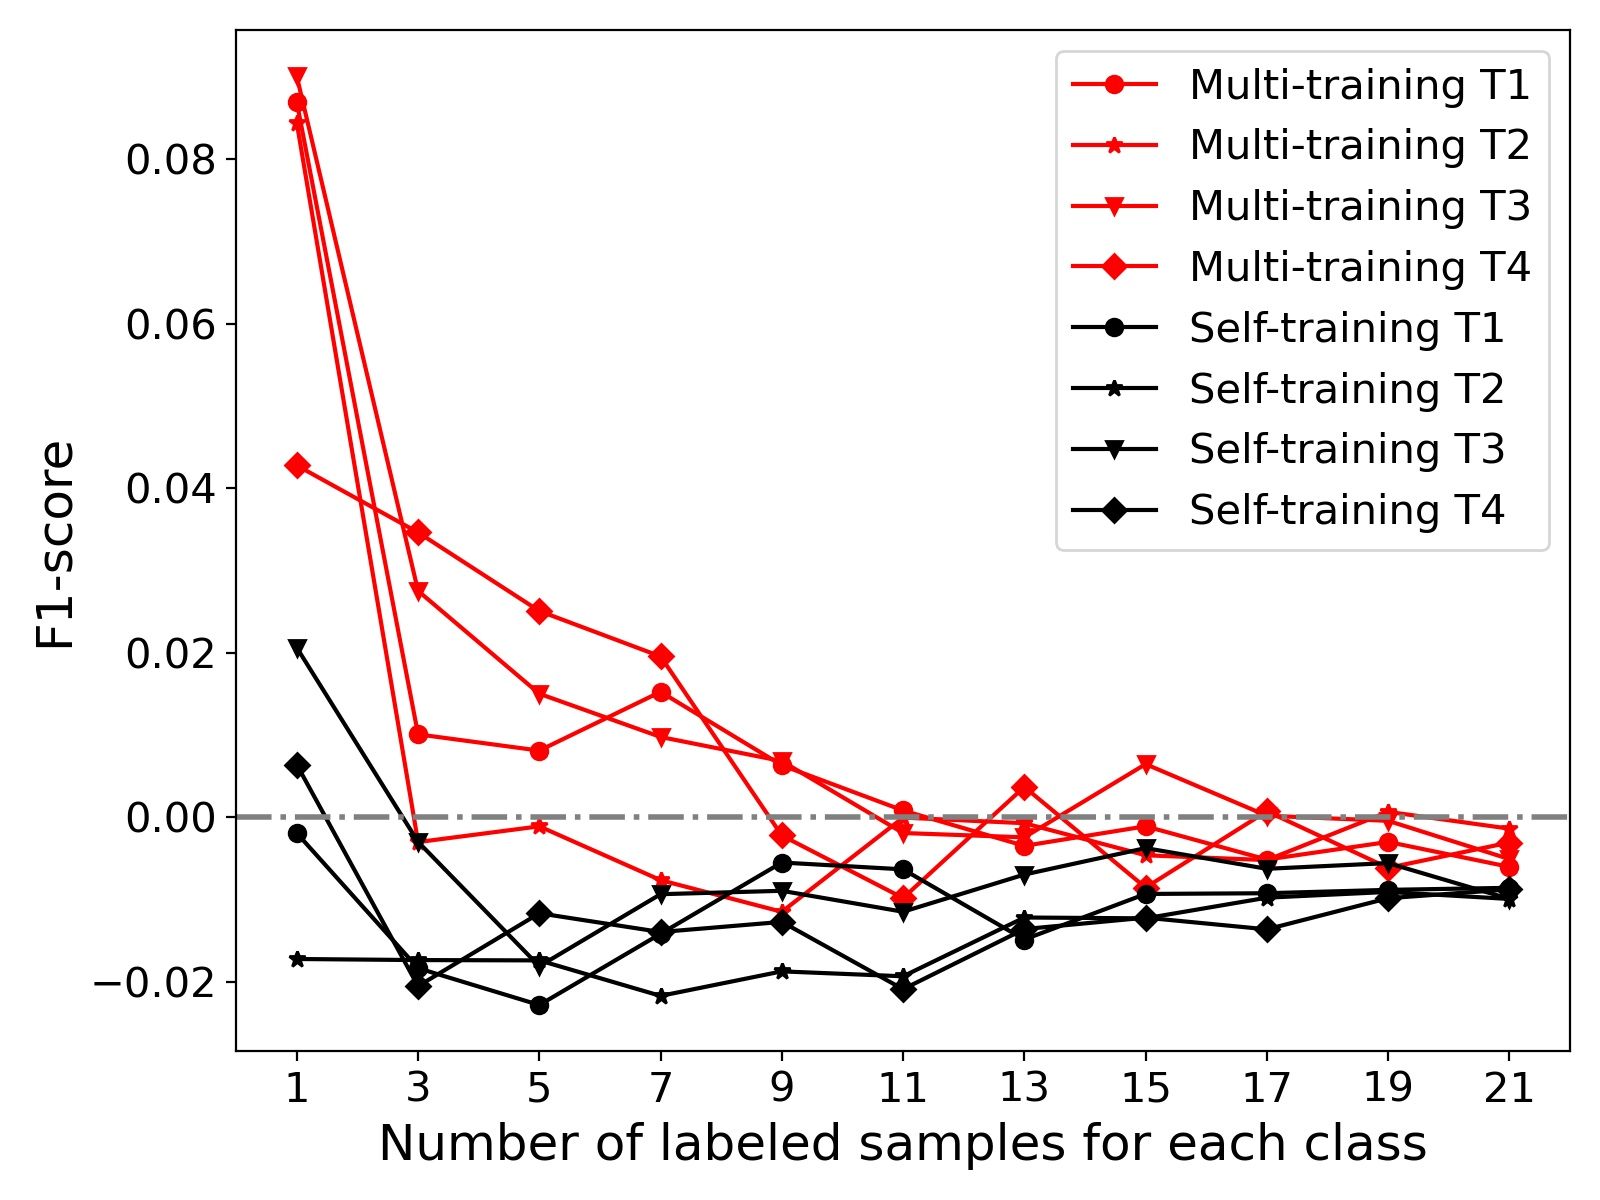
\includegraphics[width=0.5\columnwidth]{figures/images/multi_self_total_unlabel5_improved_trend_mean.jpg}
		%\caption{fig2}
	}%
	\subfigure[pic2.]{
		\centering
		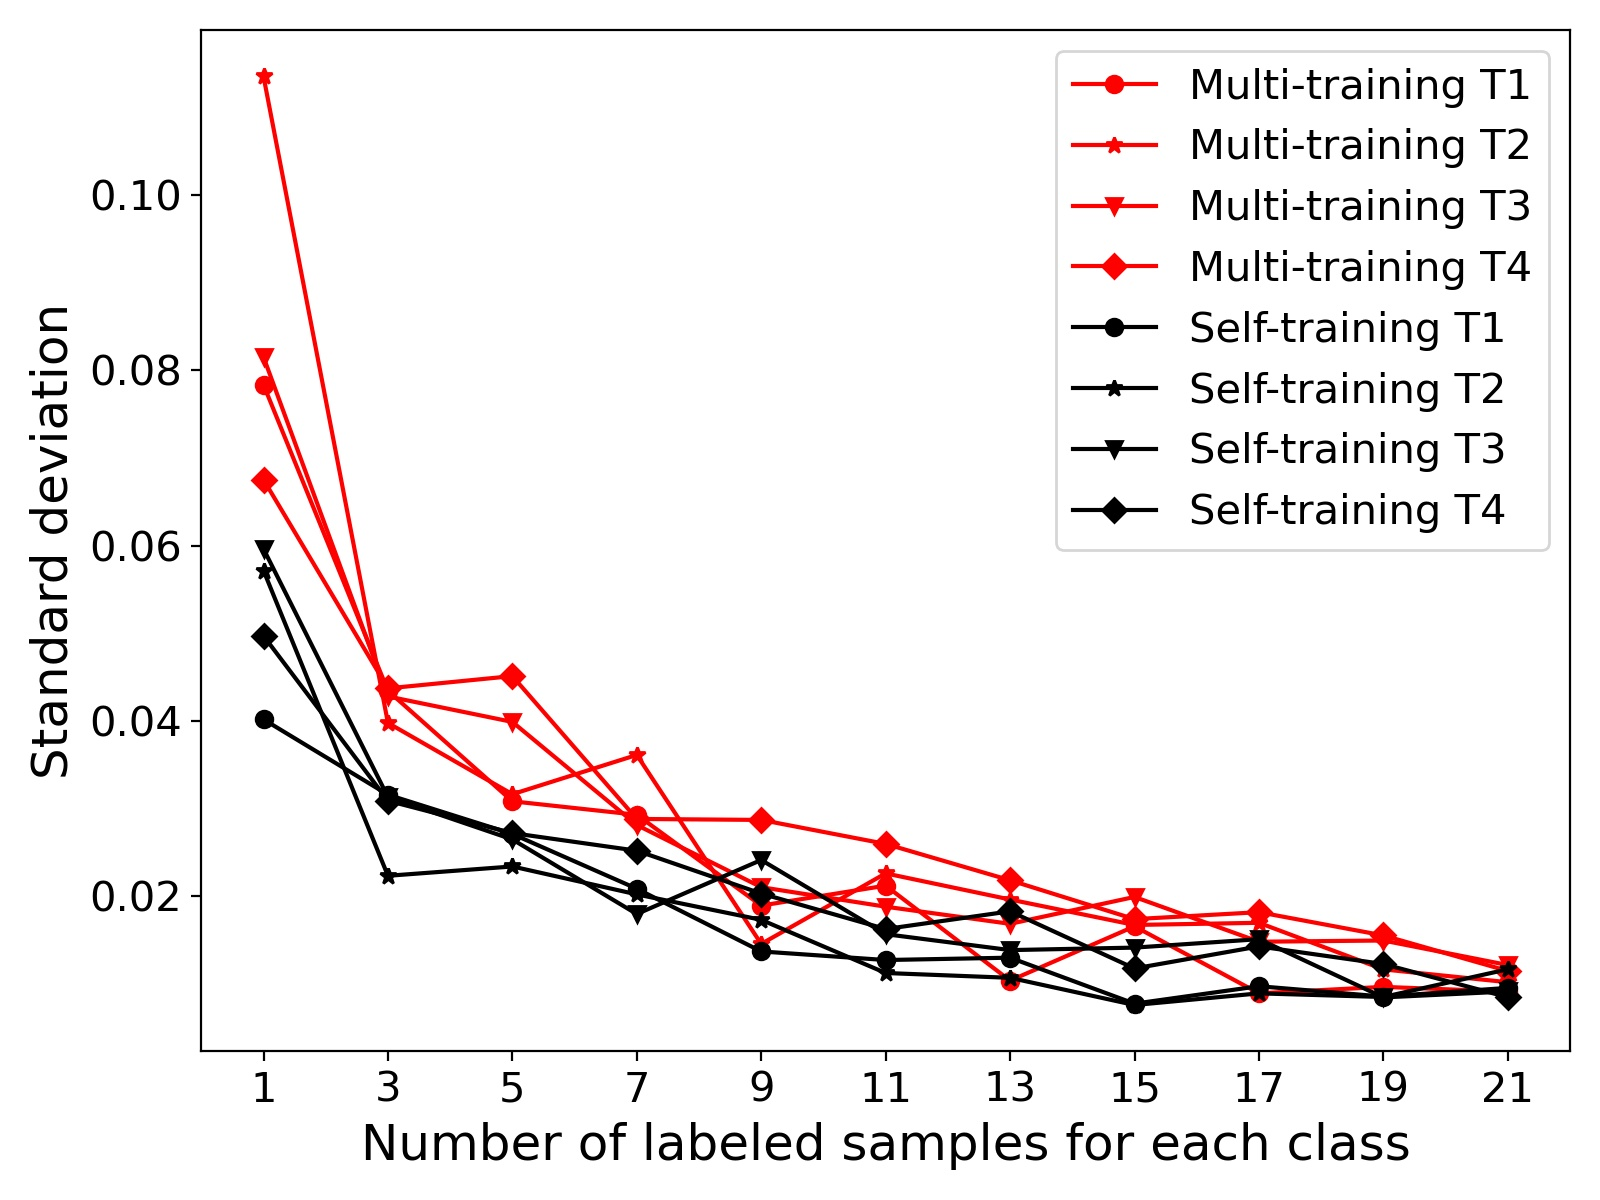
\includegraphics[width=0.5\columnwidth]{figures/images/multi_self_total_unlabel5_improved_trend_std.jpg}
		%\caption{fig2}
	}%
	
	\centering
	\caption{ pics}
\end{figure*}
In general, the F scores of vegetation and total gradually increase when Nl increases. Under the same time phase, the f scores of multi-training is always bigger than of the self-training, which to show proposed method has a great advantage over the self-training method. In particularly, when Nl is under the 5, the f score of multi-training is much more higher than of the self-training, which can be explained by that multi-training combined four time phases and extracted the features of all of them to make a better classification performance. In addition, the standard deviation of multi-training is smaller than of self-training, particularly when the Nl is under 5. This phenomenon can be observed in all four time phases.

The e, f, g, h shows the improvement of F score and standard deviation after the iterative training. The performance of multi-training is greater than of self-training in all cases. When Nu is under 5, the f score improvement and standard deviation improvement of multi-training is quite big. While with the increasing of Nl, the gap of  improvement between multi-training and self-training is narrowing. This can be explained by the sufficient Nl offered enough features to support to train the classifier in self-training. 

Fig. 11 shows the F scores and standard deviation based on different Nu and Nl. We can see that: (1)If the Nu is fixed, approximately, f score is going greater and standard deviation is going smaller by the increasing of Nl; (2)If the Nl is fixed, It's not that the bigger Nu, the higher F. To achieve the greatest F score and smallest standard deviation, Nu and Nl need to match with each other. In addition, Nu is always need to be greater when Nl increase. 

\begin{figure}[ht!]
	\centering
	
	\subfigure[pic1.]{
		\centering
		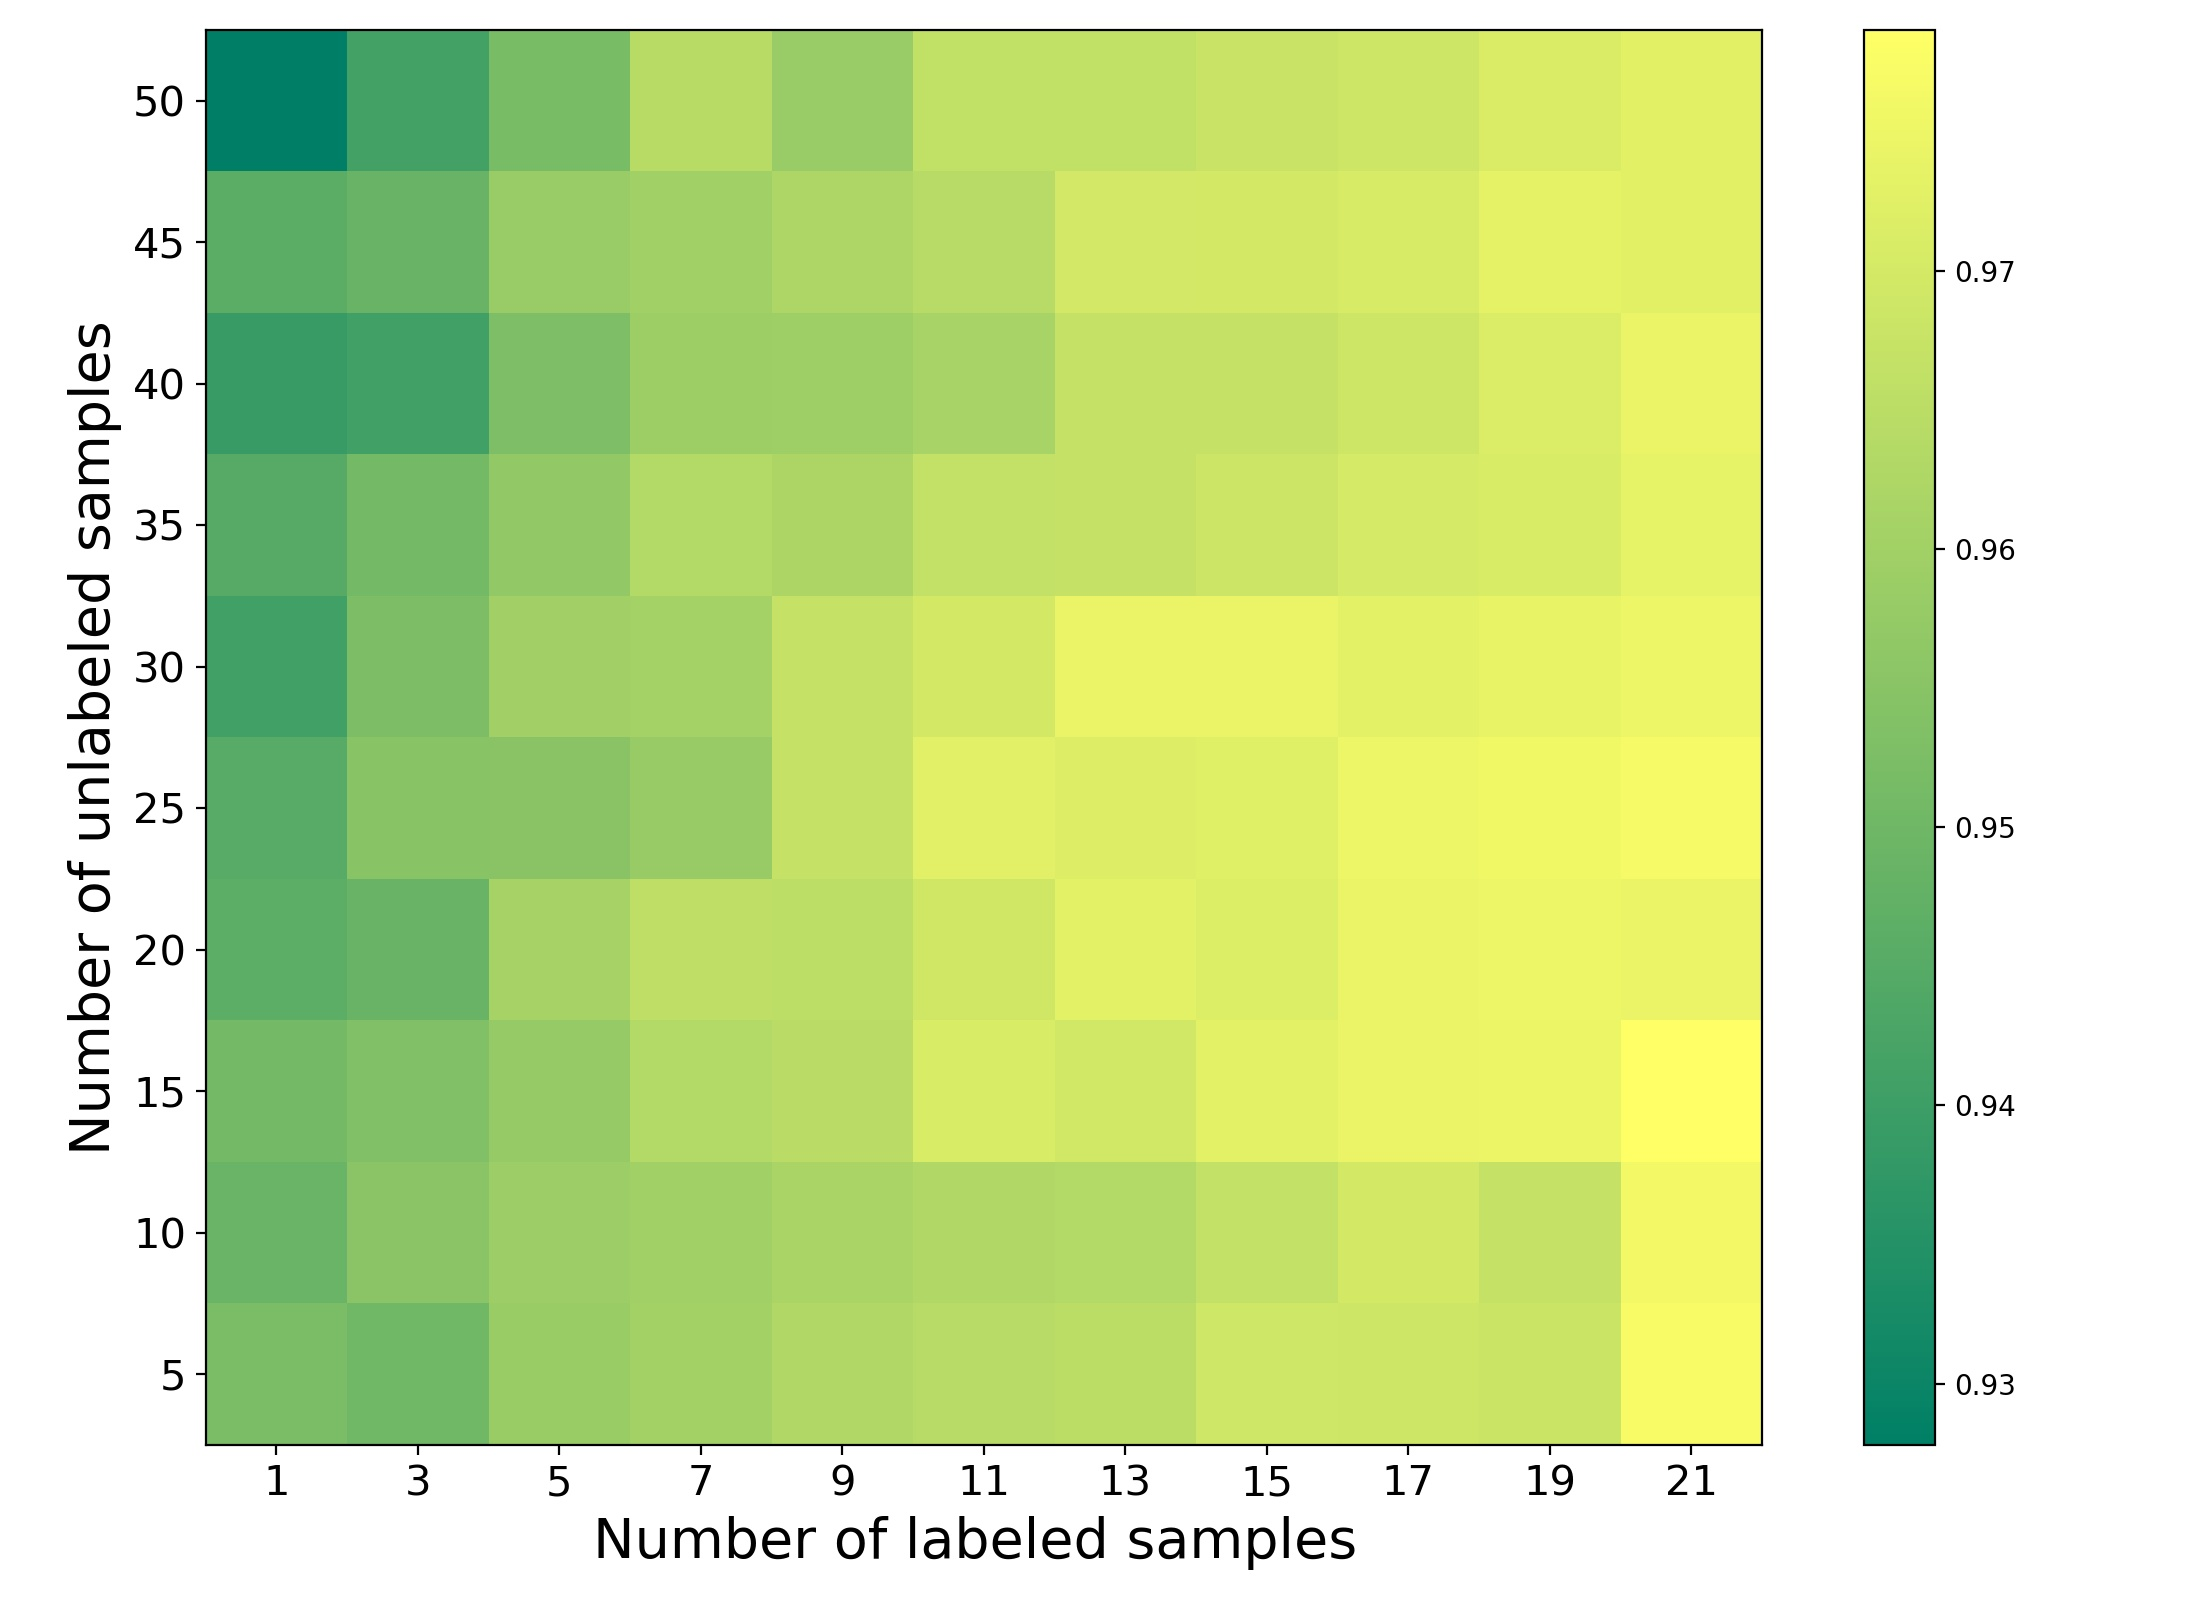
\includegraphics[width=0.5\columnwidth]{figures/images/labelunlabelplot_veg_final_mean.jpg}
		%\caption{fig1}
	}%
	\subfigure[pic2.]{
		\centering
		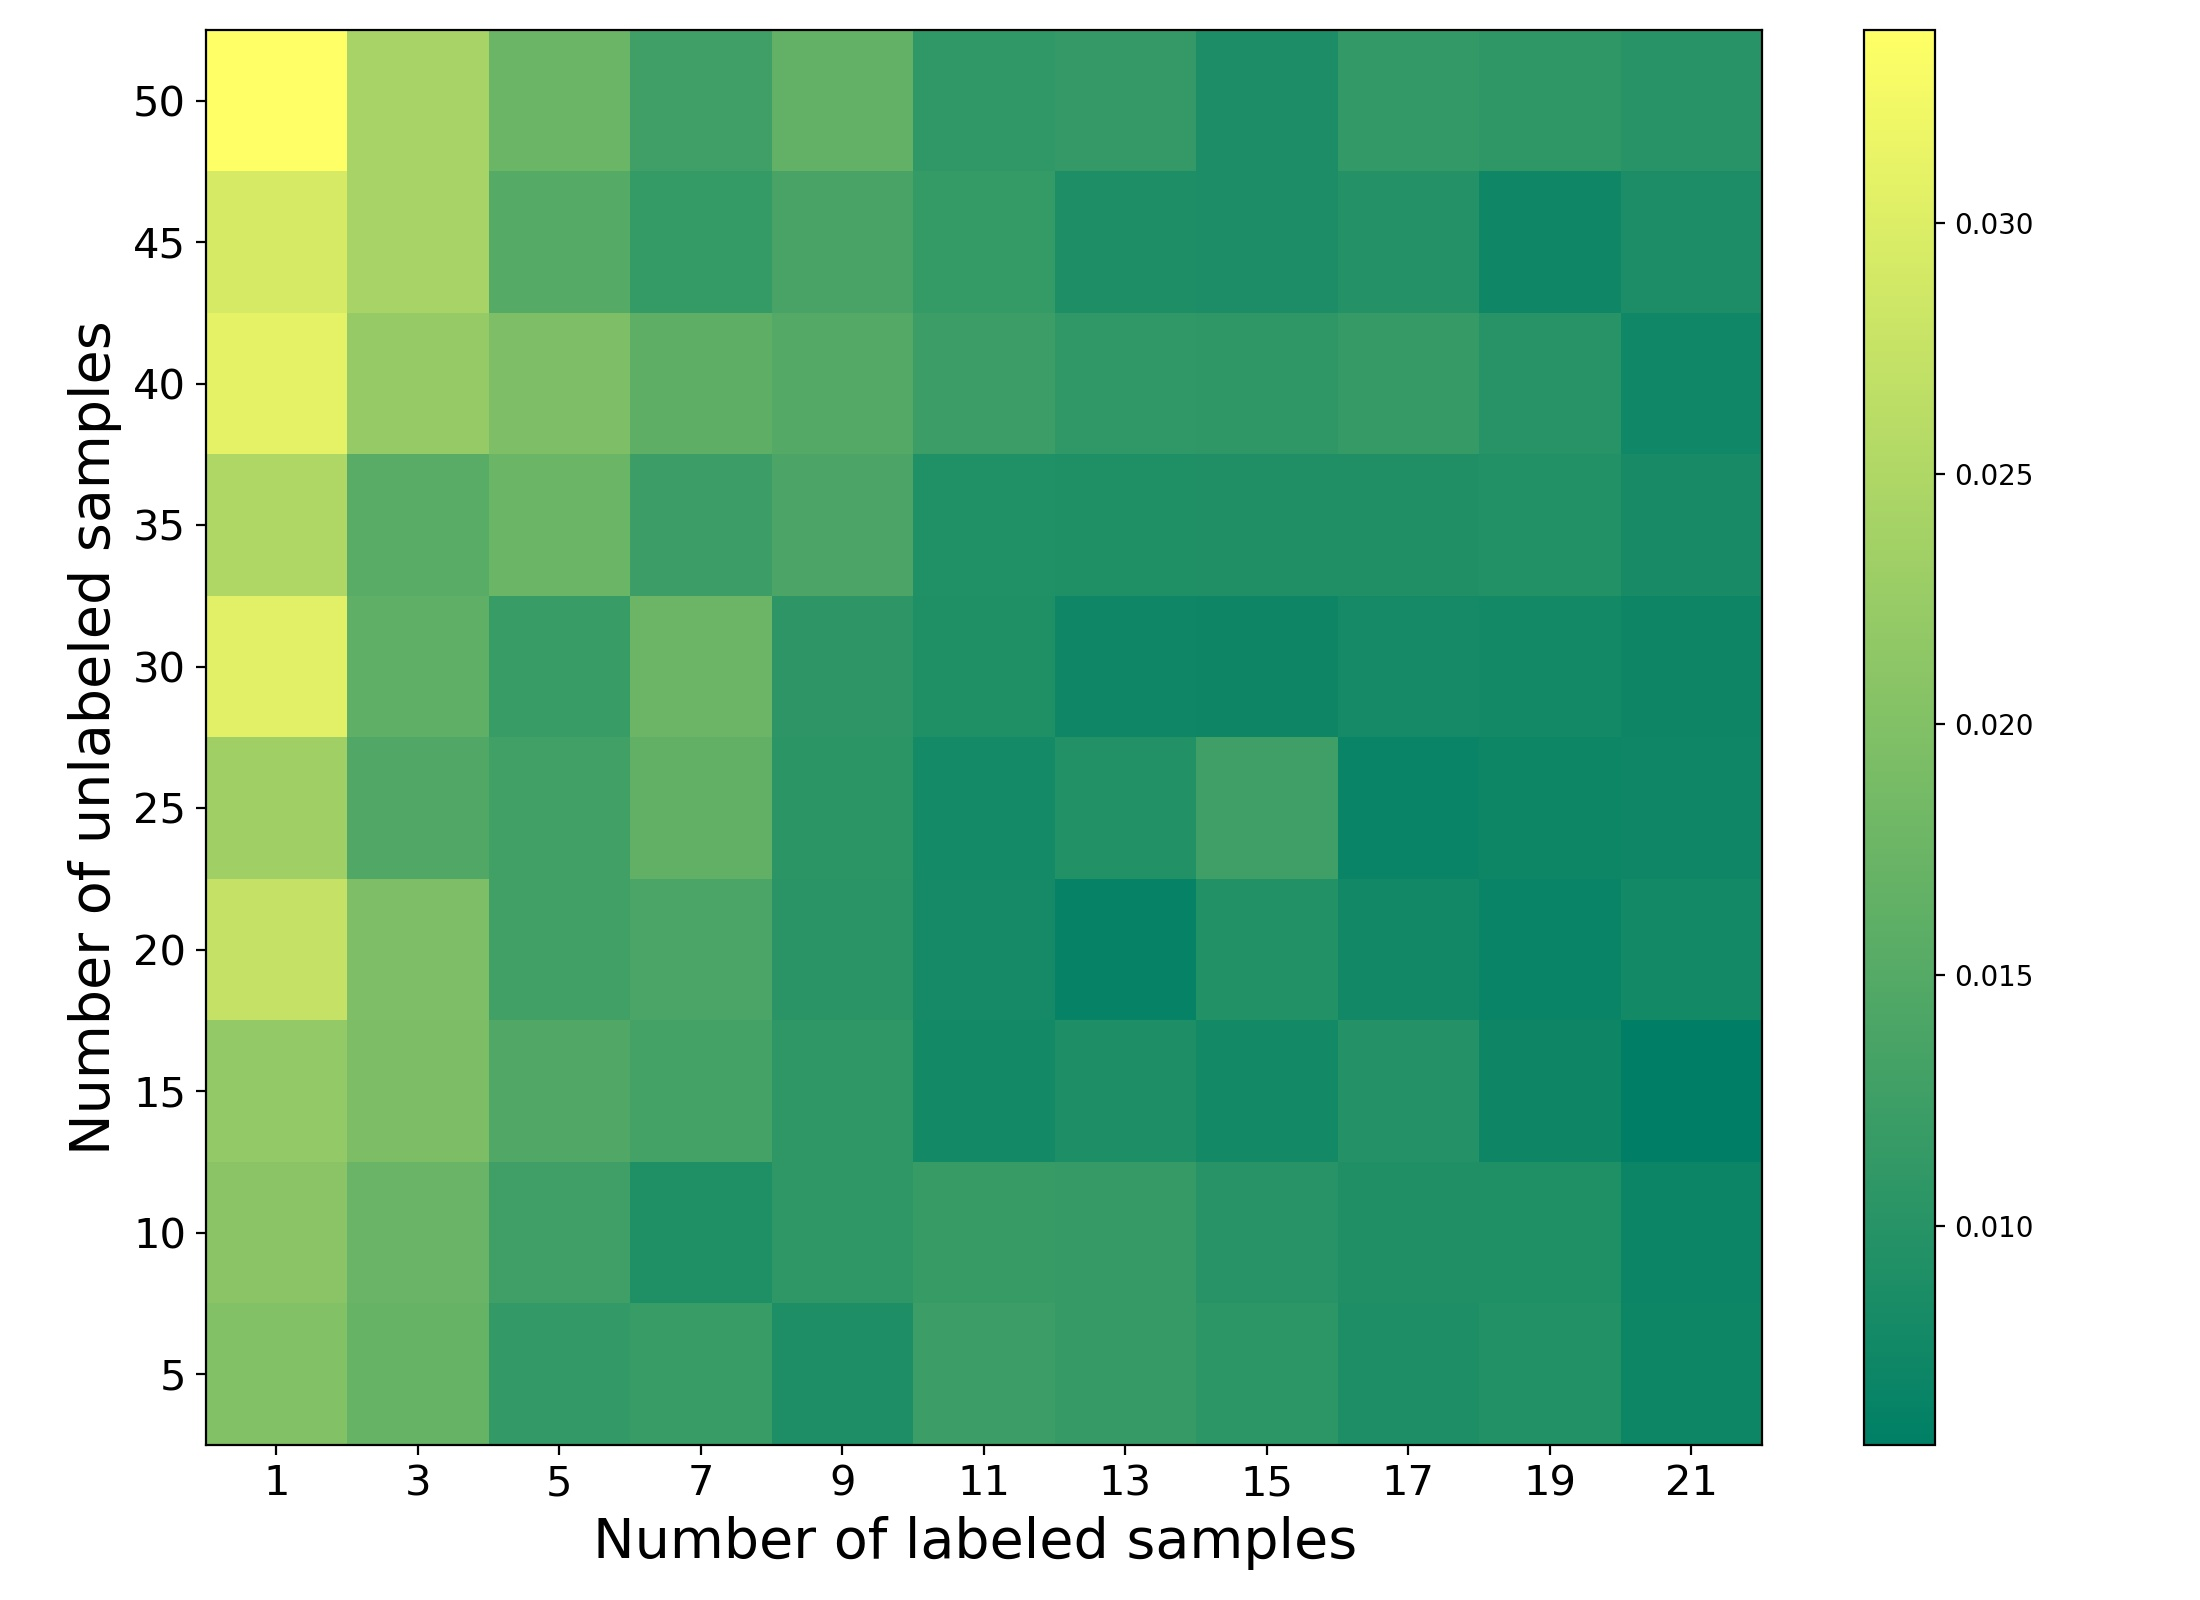
\includegraphics[width=0.5\columnwidth]{figures/images/labelunlabelplot_veg_final_std.jpg}
		%\caption{fig2}
	}%
	\quad
	\subfigure[pic3.]{
		\centering
		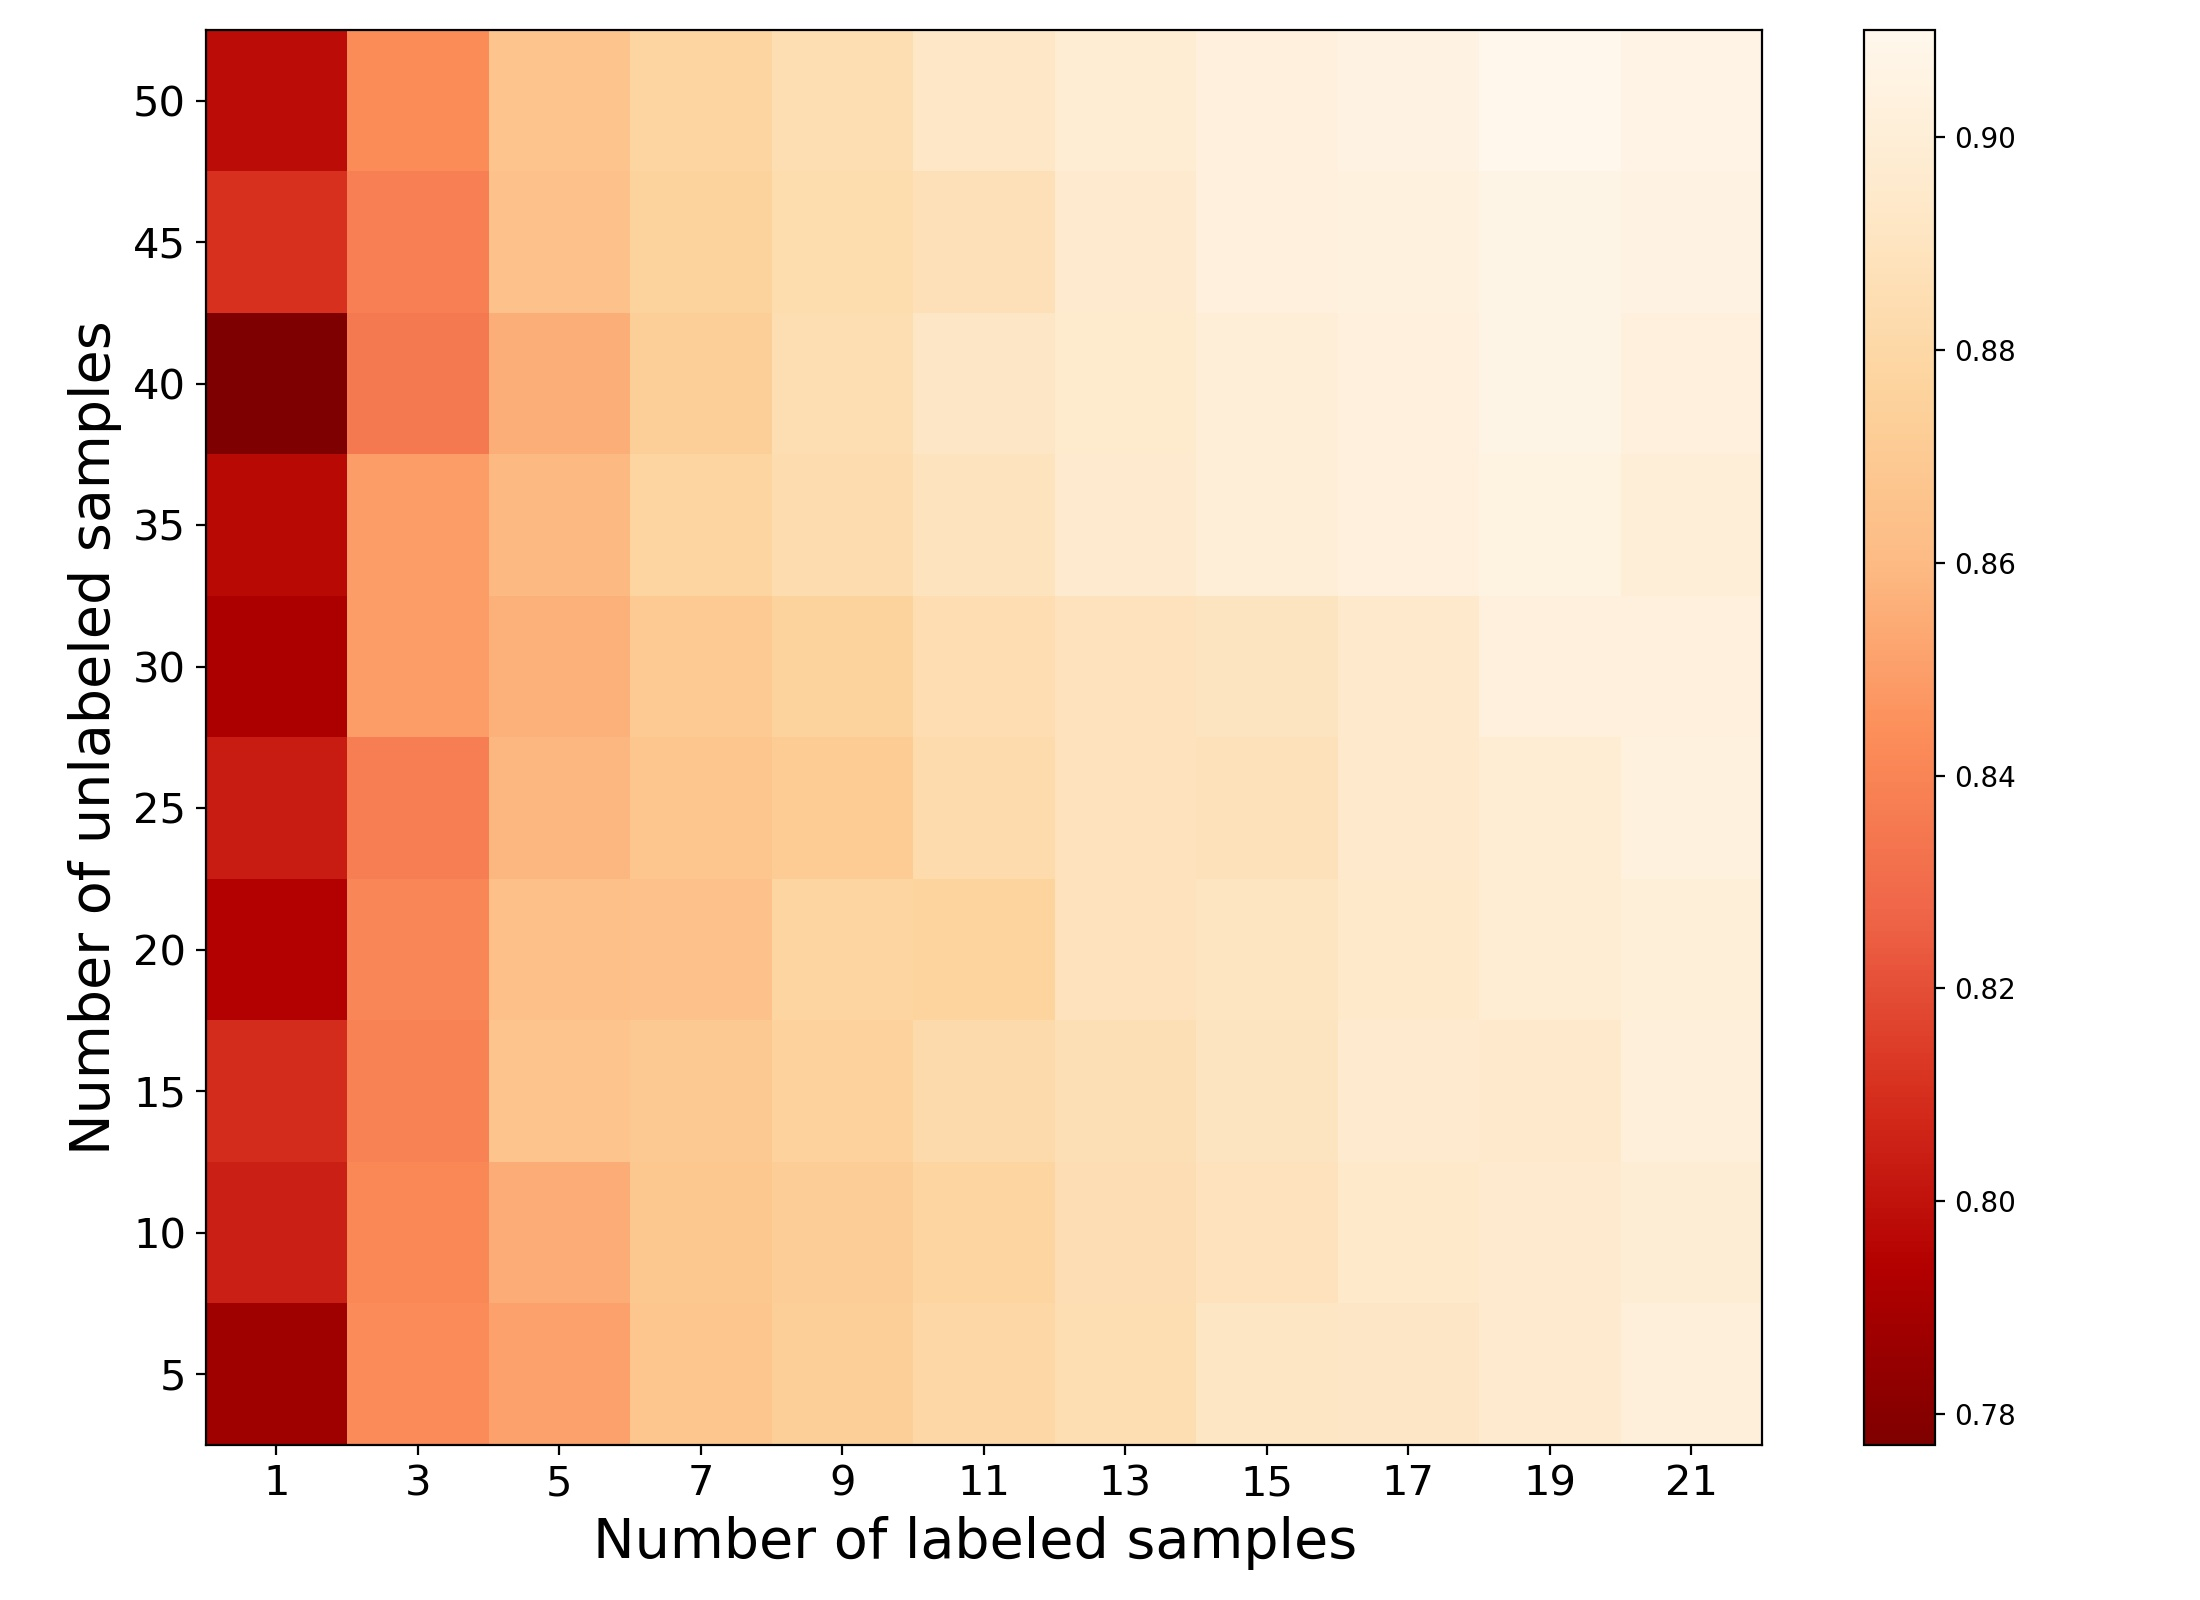
\includegraphics[width=0.5\columnwidth]{figures/images/labelunlabelplot_total_final_mean.jpg}
		%\caption{fig2}
	}%
	\subfigure[pic4.]{
		\centering
		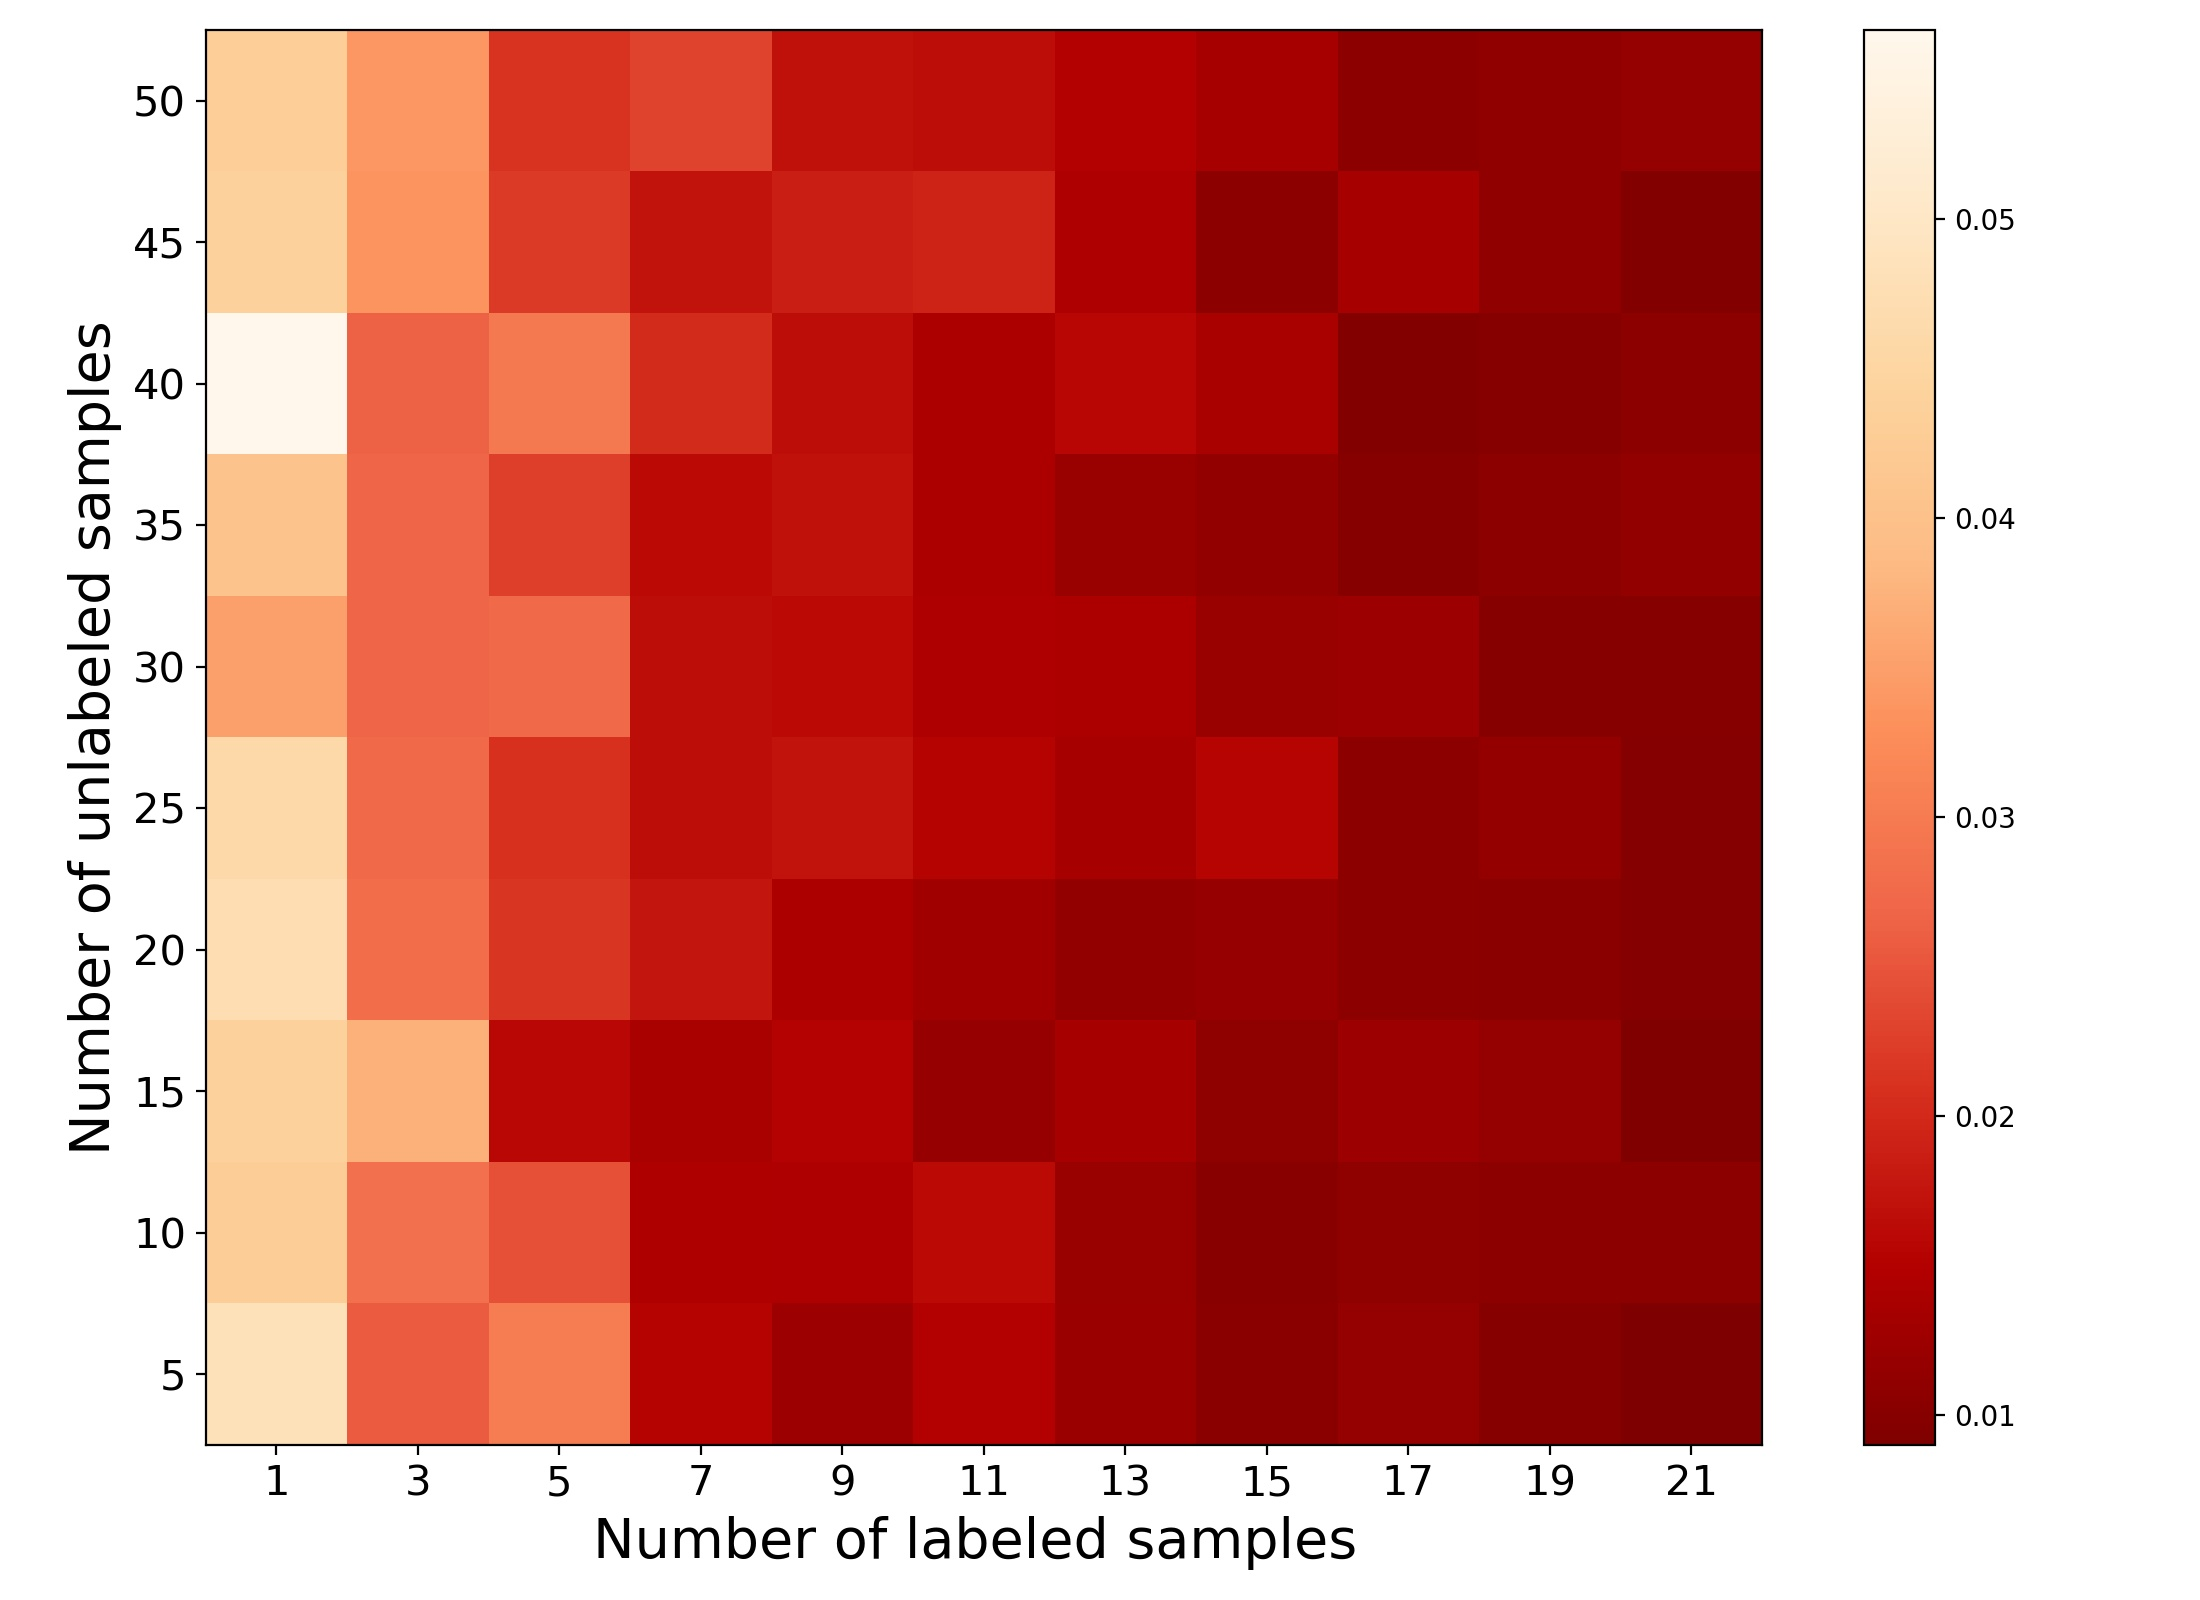
\includegraphics[width=0.5\columnwidth]{figures/images/labelunlabelplot_total_final_std.jpg}
		%\caption{fig2}
	}%
	
	\centering
	\caption{ pics}
\end{figure}

\subsection{ Influence of different number of phases}

\begin{figure}[ht!]
	\begin{center}
			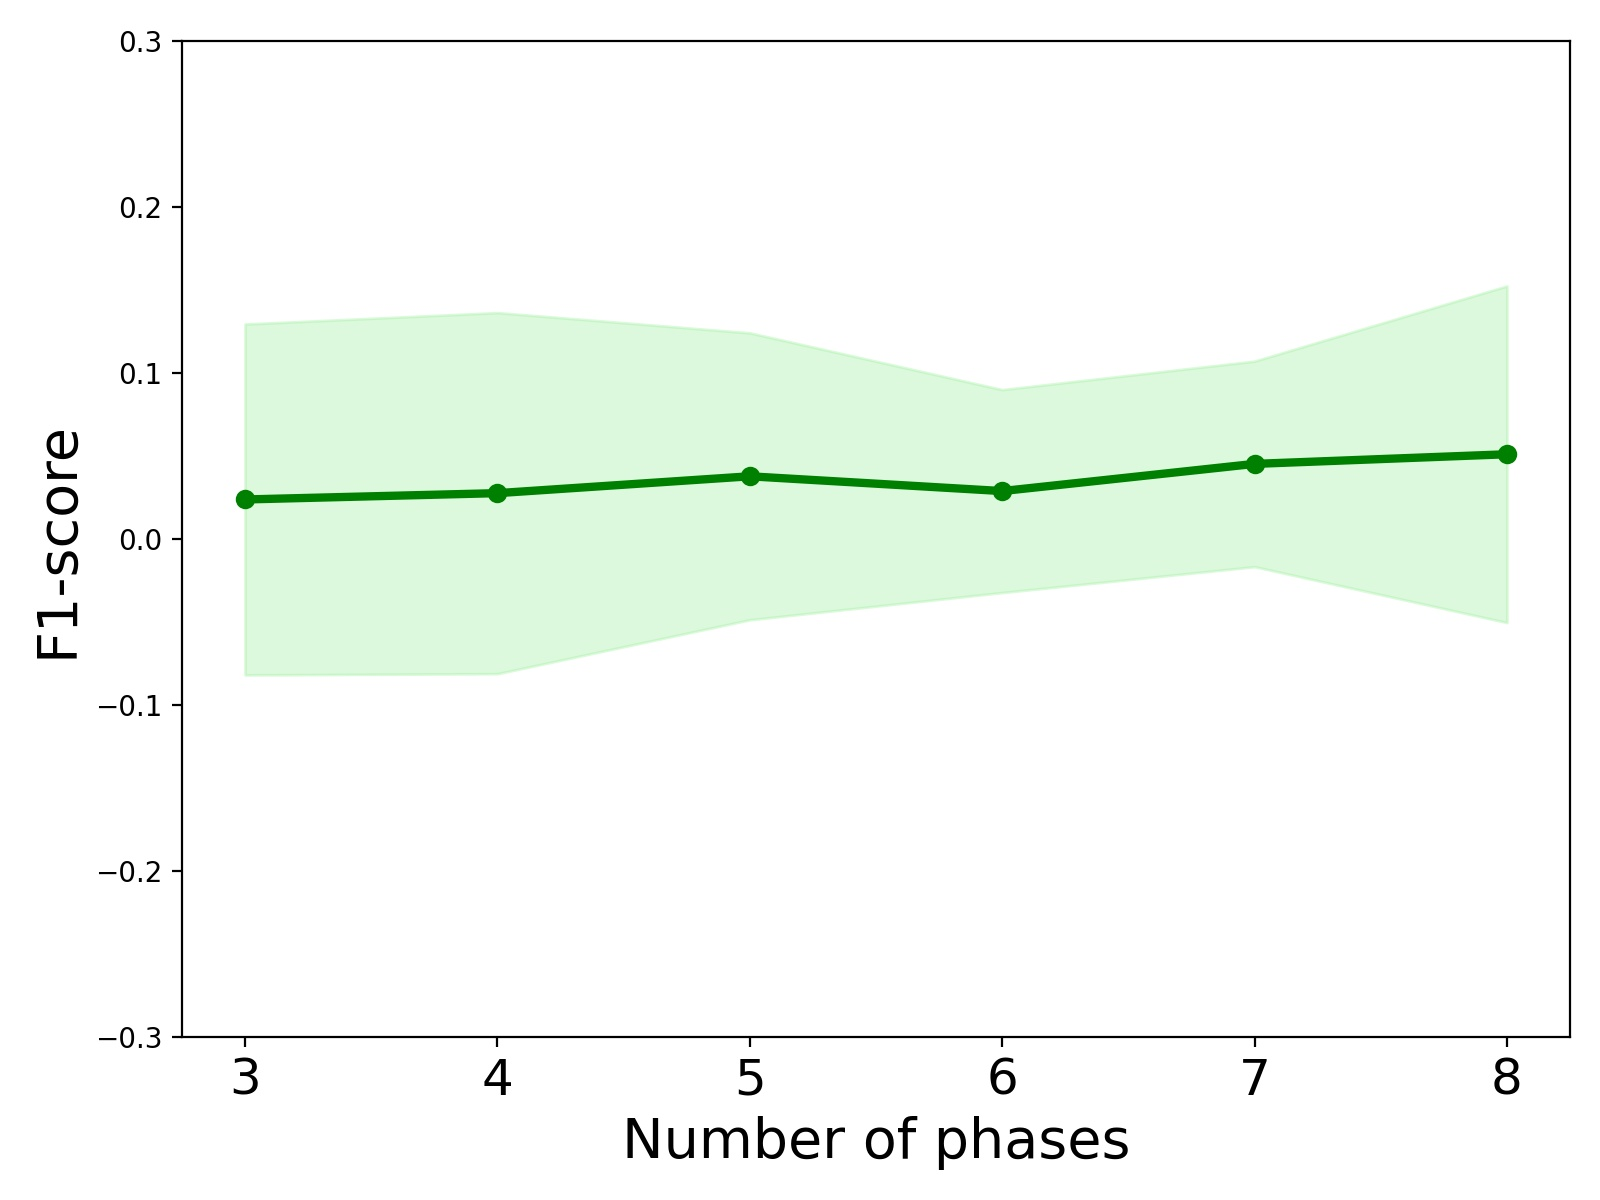
\includegraphics[width=1.0\columnwidth]{figures/images/numberOfPhasesCompareVegImprovedMean_fill.jpg}
		\caption{Figure placement and numbering}
	\label{fig:studyArea}
	\end{center}
\end{figure}

Because our algorithm is designed for multi-temporal remote sensing images’ vegetation extraction, the number of time phases will affect the performance of the algorithm. The number of time phases is modified from 3 to 8 in our experiment, and the adjacent phases are separated from each other for two to three months to explore the trend of F1-score and standard deviation. From the results, we can see that with the increase of time phase number, the average improved F1-score of vegetation extraction increases obviously, from 2 percentage points under 3 time phase to 5 percentage points under 8 time phase. This result can be explained by the equation.1. The criterion of confidence in our algorithm is provided by the prediction results of classifier on multiple time phases. We relax the equation to its up-bound which is the predicted probabilities’ average value. 

\begin{equation}
    \frac{(\prod\limits_{i=1}^kP_i)^{\frac{2}{k}}}{\frac{1}{k}\sum\limits_{i=1}^kP_i}\le \frac{(\frac{1}{k}\sum\limits_{i=1}^kP_i)^2}{\frac{1}{k}\sum\limits_{i=1}^kP_i}=\frac{1}{k}\sum\limits_{i=1}^kP_i
\end{equation}
When phases’ number increases, the variance decreases and the average stabilizes. The increase of the number can make the result more robust, which is beneficial to the judgment of the unchanged area and the selection of unlabeled samples when updating the training set. The increasing number of phases makes the algorithm more stable, so that the multi-training coincides with its original intention. The further improvement with the increase of the number of phases is the characteristic that the general algorithm considers the single phase in isolation does not have.

\section{Discussions}\label{sec:Discussions}

The core principle behind our algorithm is also ensemble learning, while it is a little different from the general idea of ensemble learning. We do not simply just combine all the classifiers own results for a set of data and then improve the final result by ensemble learning. Instead, the idea of ensemble learning in our experiment is used to provide higher confidence for the update of training samples in semi-supervised learning. Especially in this problem setting, the multi-temporal remote sensing images give our algorithm the condition of natural multi-view learning. The similarity of the data makes the results of the model under each phase in our algorithm have more reference value, and the difference of data distribution provides each model more disagreement. In the process of determining the updated sample, the discriminant formula of the algorithm is integrated into the idea of harmonic average, so that the joint confidence of all classifiers takes into account the prediction results of each classifier. But it is only regarded as a reference basis, rather than directly concluding the label of unknown data to add into the training set. Until all the samples have completed the joint confidence computing, and then training set will be updated. Considering the information of the whole image, it is more stable than the general ensemble learning. Therefore, the spatial consistency of classification results is higher than that of general integrated learning.

\begin{figure}[ht!]
	\begin{center}
			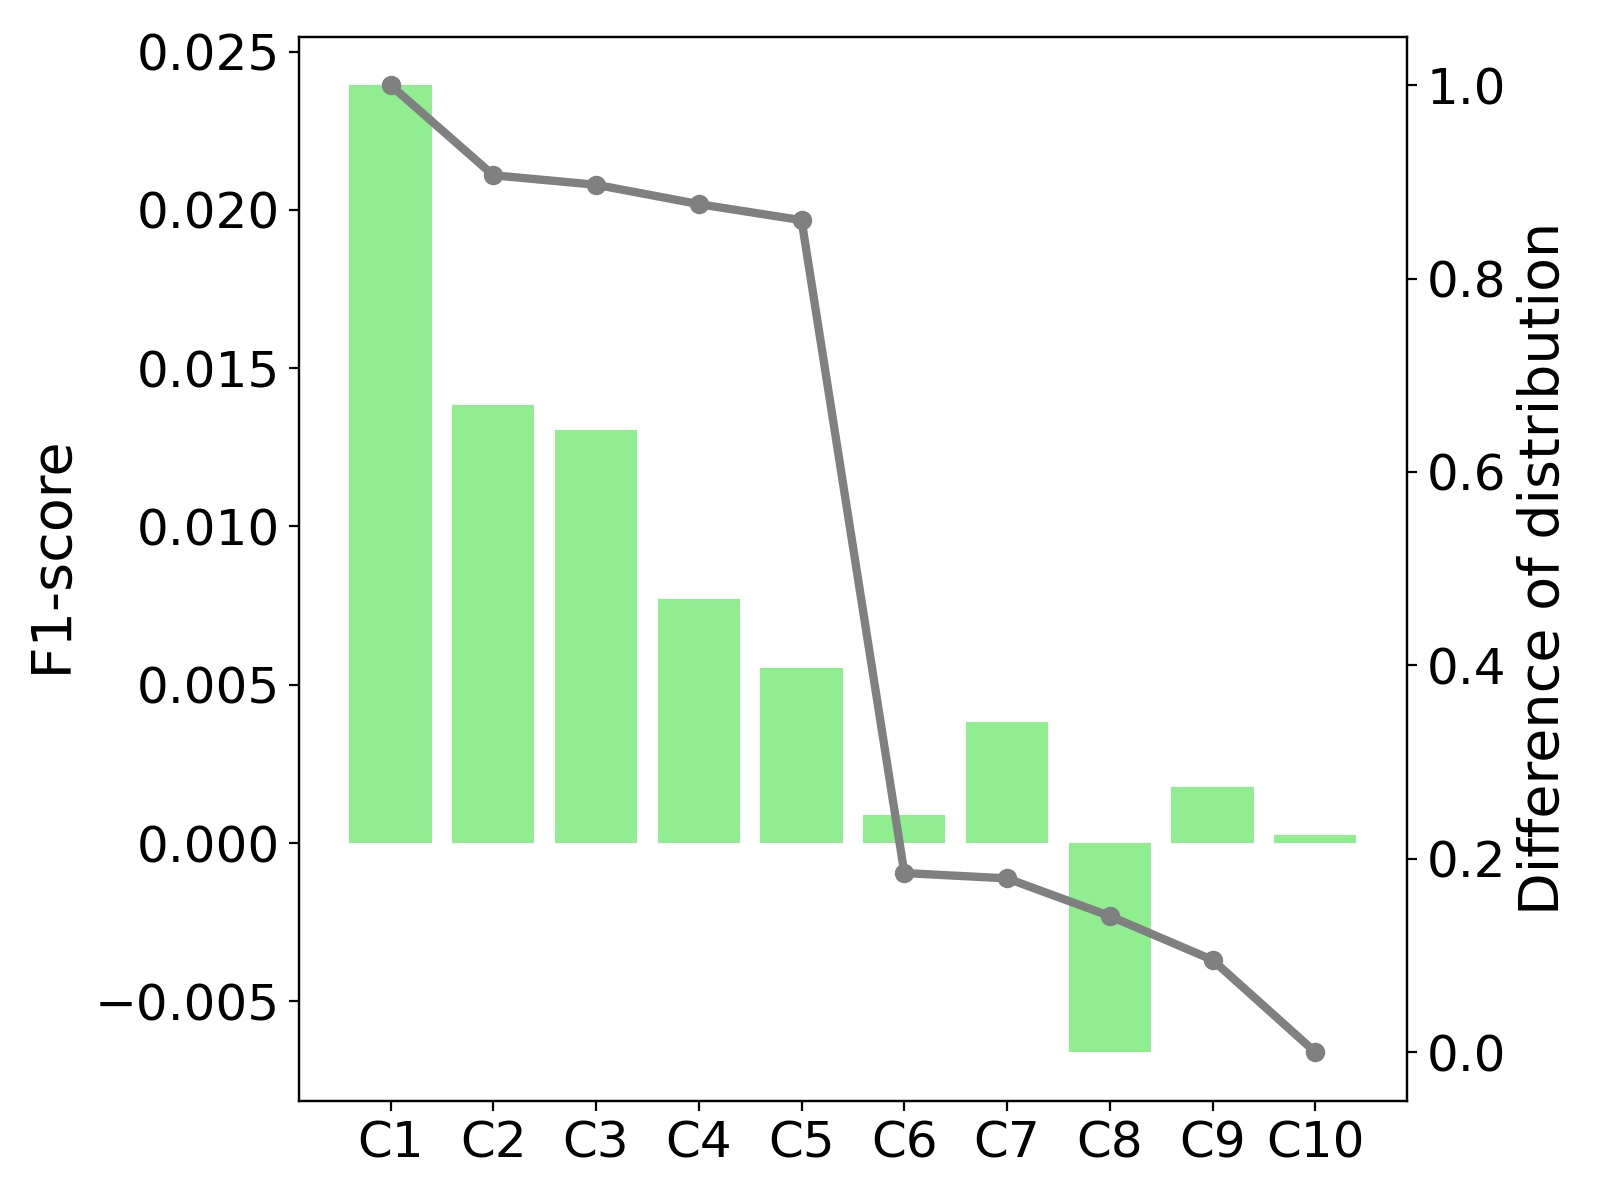
\includegraphics[width=1.0\columnwidth]{figures/images/yearsdiff_compare_multiself_vegimprove_label3unlabel5.jpg}
		\caption{Figure placement and numbering}
	\label{fig:studyArea}
	\end{center}
\end{figure}
In order to excavate the deeper law of our proposed method, we design an experiment on the influence of different time-phase combination data’s distribution on multi-temporal training to improve classification accuracy. We firstly calculate the difference of data distribution directly for the existing data of multiple time phases. Because our algorithm is for multi-temporal training, just computing the difference of two time-phase data distribution can not represent the difference of the combination’s data distribution difference. Therefore, we use the following formula to calculate the difference:

\begin{equation}
	Diff(D_1,D_2,\dots,D_k)=\frac{1}{N}(\sum\limits_{j=1}^{N}(\frac{1}{f}\sum\limits_{i=1}^{N}std(x_{1}^{(f)},x_{2}^{(f)},\dots,x_{k}^{(f)})))
\end{equation}

This calculation method takes into account the difference between multiple phase, and satisfies the setting of the problem. We choose the first five time-phase combinations with the largest distribution difference and the five combinations with the smallest distribution difference. For each combination of multiple-phase data, the algorithm designed above is applied to compare the classification accuracy improved of each combination.

As the figure above show, there is a high correlation between the difference of data distribution and the improvement of the accuracy of the final classification results. The greater the difference in combination’s data distribution, the better the effect of the algorithm. Let us consider from the perspective of multiple classifiers learning and communication. In the early stage of training, the classifiers under each phase learn only the distribution of their own data, but with a global communication at the end of each round, each classifier has opportunity to implicitly learn the distribution of other phase data. According to the whole data distribution, new training samples are selected randomly to correct their original parameters in order to obtain more accurate and consistent classification results. If the difference of data distribution is too tiny, the parameters of each classifier are almost the same in the above communication process, so it is impossible to obtain additional new information from other phases and it can not improve the accuracy. From the point of view of information theory, it is assumed that the initial classification performance of  based classifier on each time is similar. When time-phase number fixed, the greater the difference of data distribution, the greater the total amount of information provided by time-phase combination to all classifiers. Correspondingly, a combination of data distributions close to the amount of information provided by a single phase, which results in that the classifier can not get more information from the training process and the performance improvement is limited.

\section{Conclusions}\label{sec:Conclusions}
In this study, a multi-temporal semi-supervised method was designed to utilize information from multi-temporal remote sensing images and classify the land use types from high-spatial and -temporal resolution remote sensing images. A sparse training set is suffificient to extract the multi-temporal vegetation and other land cover collectively. Particularly, this method exploits the difference between the observed spectral distributions of four images in a mutual learning way, providing a new strategy to deal with multi-temporal image classifification. The scalability and mobility of this work are very good, such as the detection of cyanobacteria in multi-temporal water bodies and the updating of land use information in time series.

\section*{ACKNOWLEDGEMENTS (Optional)}\label{ACKNOWLEDGEMENTS}
Acknowledgements of support for the project/paper/author are welcome. 

{
	\begin{spacing}{1.17}
		\normalsize
		\bibliography{ISPRSguidelines_authors} % Include your own bibliography (*.bib), style is given in isprs.cls
	\end{spacing}
}


\section*{APPENDIX (Optional)}\label{APPENDIX}

Any additional supporting data may be appended, provided the paper does not exceed the limits given above. 

\vspace{1cm}
\textit{Revised January 2020}

\end{document}
